% ch4-bessel.tex
\documentclass[../main/main]{subfiles}

\begin{document}

\chapter{Bessel関数}


\vspace{-180pt}
\begin{figure}[H]
  \begin{flushright}
    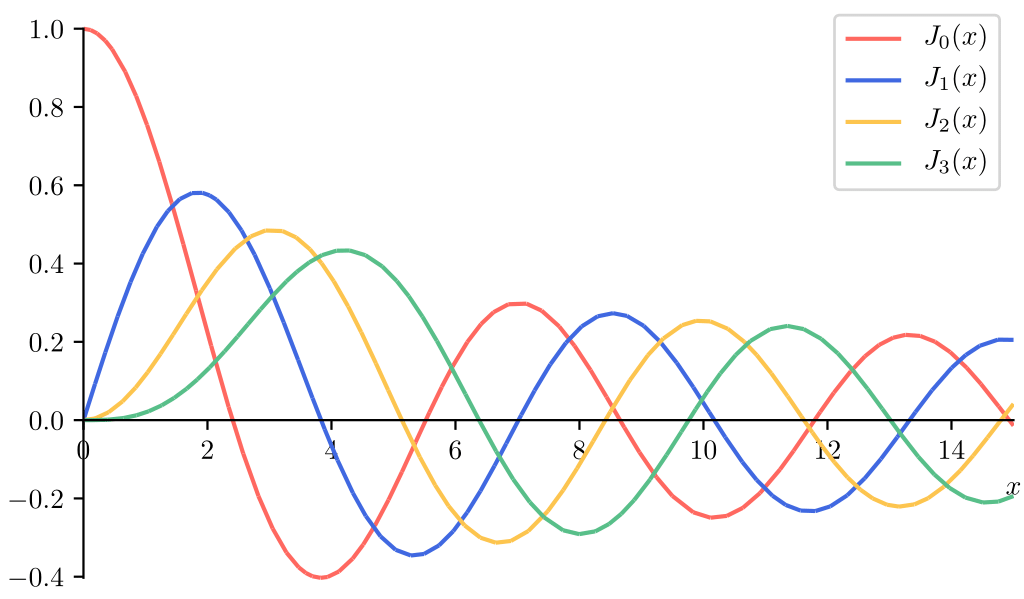
\includegraphics[width=80mm]{../fig/bessel/bessel_title.png}
  \end{flushright}
\end{figure}
\small

\vspace{-12pt}
\footnotesize
Bessel関数は円対称な系における波動・振動を解析するときなどに必ずといってよいほど出現し、
物理学のみならず工学の諸分野においても頻繁に応用される。
そのため、Bessel関数はこれまで扱ってきた特殊関数と比べてはるかに重要度が高い関数であるといえる。
ひとことで言えばBessel関数$J_\nu(x)$とはBesselの微分方程式
\begin{equation*}
  y^{\prime\prime} + x y^\prime + (x^2 - \nu^2)y = 0
\end{equation*}
の基本解のひとつなのであるが、多くの物理現象ではこれと線形独立なもうひとつの解も重要視される。
さらにこれと関連する変形Bessel関数も拡散現象を記述する際に必要に迫られ、
またBessel関数の特殊な場合である球Bessel関数も球対称な現象を記述する際に重要となる。
このようにBessel関数には関連する関数が多いため、他の特殊関数と比べて内容が多くなっているが、
それぞれの導出に必要な計算は比較的軽めになっている。
ぜひ自分で手を動かして公式の体系を把握し、これらの関数に慣れ親しんでいきたいところである。

\small

\section{Bessel関数}
\subsection{整数次のBessel関数(第1種Bessel関数)}

整数次のBessel関数(第1種Bessel関数)$J_n(x)$を母関数\eqref{eq:Jn-gene}により定義する。
一般項や漸化式、微分方程式の導出方法はこれまでに扱った特殊関数とほとんど同様にして導ける。
積分表示\eqref{eq:Jn-integral}が新たに登場しているが、
この式の導出方法は二次元の円盤のFourier変換を計算する際に重要になる ( 問題 [4-1] )。

\subsubsection*{公式集}

\vspace{12pt}
\paragraph{母関数(定義)}
\begin{equation}\label{eq:Jn-gene}
  g(t, x) = e^{\frac{x}{2} \( t-\frac{1}{t} \)} 
	= \sum_{n=-\infty}^\infty J_n(x) t^n
\end{equation}

\paragraph{母関数II}
\begin{equation}\label{eq:Jn-gene2}
  g(\theta, x) = e^{ix\sin\theta}
	= \sum_{n=-\infty}^\infty J_n(x) e^{in\theta}
\end{equation}

\paragraph{偶奇性}
\begin{equation}\label{eq:Jn-guki}
  J_n(-x) = (-1)^n J_n(x) 
\end{equation}

\paragraph{負の整数次}
\begin{equation}\label{eq:Jn-fu}
  J_{-n}(x) = (-1)^n J_n(x)
\end{equation}

\paragraph{$x=0$での特殊値}
\begin{equation}
  J_n(0) = 
  \left\{ 
  \begin{alignedat}{2}
    &1 &\qquad	& (n=0) \\
    &0 &			& (n\neq 0)
  \end{alignedat}
  \right.
\end{equation}

\paragraph{Bessel関数の級数}
\begin{gather}
  \sum_{n=-\infty}^\infty J_n(x) = 1 \\
  J_0(x) + 2 \sum_{n=1}^\infty J_n(x) = 1
\end{gather}

\paragraph{Besselの積分表示}
\begin{equation}\label{eq:Jn-integral}
  J_n (x) = \frac{1}{2\pi} \int_{-\pi}^\pi \cos (n \sin \theta -n\theta ) d\theta
\end{equation}

\paragraph{一般項}
\begin{equation}\label{eq:Jn-ippan}
  J_n(x) = \sum_{i=0}^\infty \frac{(-1)^i}{i! (n+i)!} \( \frac{x}{2} \)^{n+2i}
\end{equation}

\paragraph{漸化式}
\begin{equation}\label{eq:Jn-req}
  \frac{2n}{x} J_n(x) = J_{n-1} (x) + J_{n+1}(x)
\end{equation}

\paragraph{微分漸化式}
\begin{equation}\label{eq:Jn-diffreq}
  2\frac{d J_n(x)}{dx} = J_{n-1}(x) - J_{n+1} (x)
\end{equation}

\paragraph{昇降演算子}
\begin{alignat}{2}
  &\mathrm{\textbf{下降演算子}} & \quad & \( \dx{} + \frac{n}{x} \) J_n(x) = J_{n-1}(x) \label{eq:Jn-kako}\\
  &\mathrm{\textbf{上昇演算子}} &  & \( \dx{} - \frac{n}{x} \) J_n(x) =  - J_{n+1}(x) \label{eq:Jn-josho}
\end{alignat}

\paragraph{微分方程式}
\begin{gather}
  \frac{d^2 J_n(x)}{dx^2} + \frac{1}{x} \frac{d J_n(x)}{dx} + \( 1-\frac{n^2}{x^2} \) J_n(x) = 0 
		\label{eq:Jn-diff-eq1}\\
  \frac{d^2 J_n(kx)}{dx^2} + \frac{1}{x} \frac{d J_n(kx)}{dx} + \( k^2 -\frac{n^2}{x^2} \) J_n(kx) = 0
		\label{eq:Jn-diff-eq2}
\end{gather}

\paragraph{自己随伴形}
\begin{gather}
  \dx{} \[ x \dx{} J_n (x) \] + \( x - \frac{n^2}{x} \) J_n(x) = 0 \label{eq:Jn-self-1}\\
  \dx{} \[ x \dx{} J_n (kx) \] + \( k^2 x - \frac{n^2}{x} \) J_n(kx) = 0 \label{eq:Jn-self-2}
\end{gather}

\paragraph{微分・積分公式}
\begin{alignat}{2}
  \dx{} [x^n J_n(x)] &= x^n J_{n-1}(x) , &  \int x^n J_{n-1}(x) dx &= x^n J_n(x) + C \\
  \dx{} [x^{-n} J_n(x)] &= -x^{-n} J_{n+1} (x) , &\quad\qquad \int x^{-n} J_{n+1} (x) dx &= - x^{-n} J_n(x) + C
\end{alignat}

% 図
\begin{figure}[tb]
\begin{tabular}{cc}
\hspace{-24pt}
 \begin{minipage}{0.50\hsize}\small
    \begin{figure}[H]
      \centering
      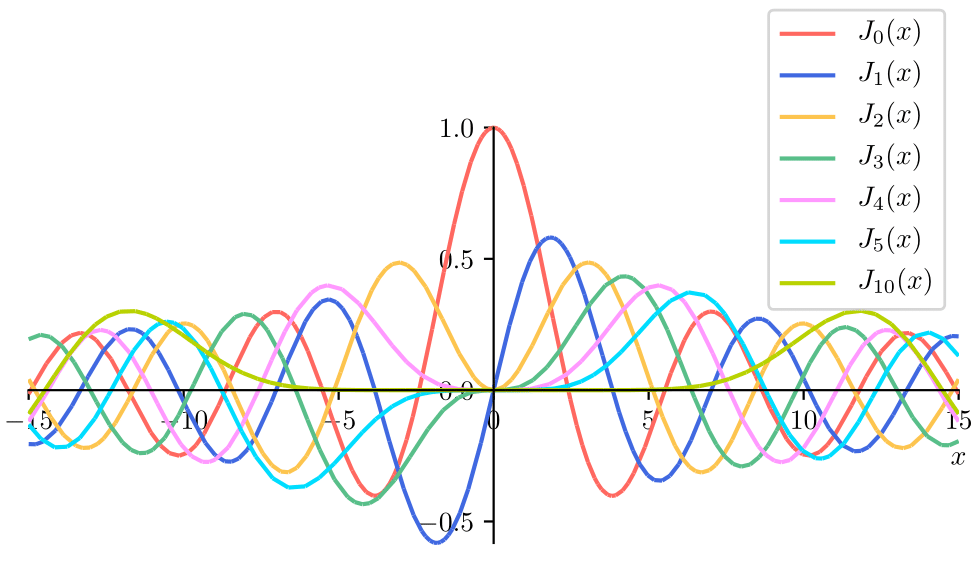
\includegraphics[width=75mm]{../fig/bessel/bessel_n.png}
    \end{figure}
 \end{minipage}

 \begin{minipage}{0.50\hsize}
    \begin{figure}[H]
      \centering
      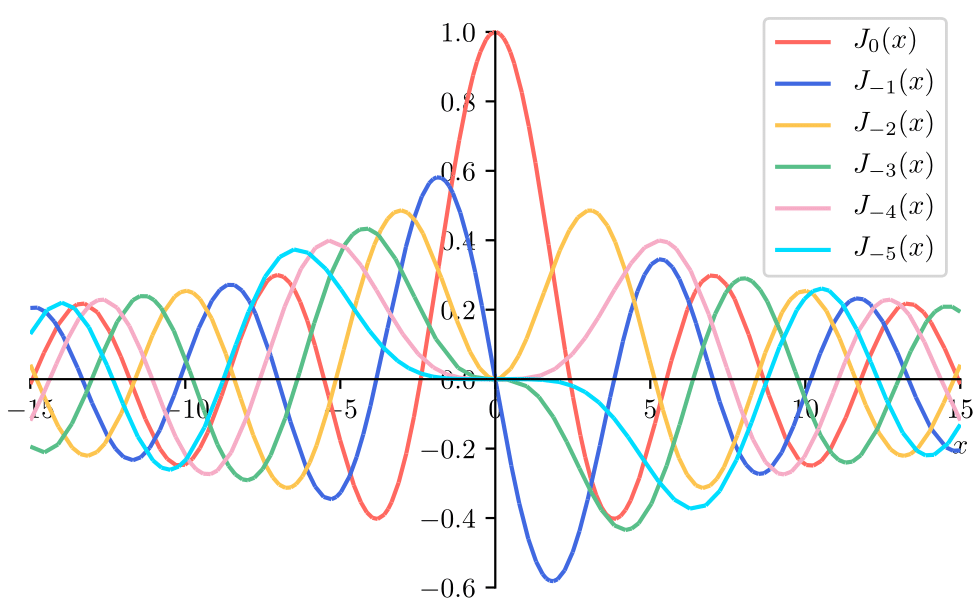
\includegraphics[width=75mm]{../fig/bessel/bessel_n_minus.png}
    \end{figure}
 \end{minipage}
\end{tabular}
\caption{	整数次のBessel関数 $J_n(x)$}
\end{figure}



\subsubsection*{証明}

\vspace{12pt}
\paragraph{母関数 $\Longrightarrow$ 母関数II}
母関数\eqref{eq:Jn-gene}で$t$を$ e^{i \theta}$と置き換えることで直ちに\eqref{eq:Jn-gene2}が得られる。
\qed

\paragraph{母関数 $\Longrightarrow$  偶奇性}
母関数\eqref{eq:Jn-gene}の中辺から$g(-t, -x) = g(t, x)$が分かるので、
\eqref{eq:Jn-gene}の右辺から
\begin{equation*}
  \sum_{n=-\infty}^\infty J_n(-x) (-t)^n = \sum_{n=-\infty}^\infty J_n(x) t^n \qquad \therefore
  \sum_{n=-\infty}^\infty J_n(-x) t^n = \sum_{n=-\infty}^\infty (-1)^n J_n(x) t^n
\end{equation*}
$t^n \ (n\in \mathbb{Z})$の係数を比較して、
\begin{equation*}
  J_n(-x) = (-1)^n J_n(x)
\end{equation*}\qed

\paragraph{母関数 $\Longrightarrow$ 負の整数次}
母関数\eqref{eq:Jn-gene}の中辺から$g(\frac{1}{t}, x) = g(-t, x)$が分かるので、
\eqref{eq:Jn-gene}の右辺から
\begin{equation*}
  \sum_{n=-\infty}^\infty J_n(x) t^{-n} = \sum_{n=-\infty}^\infty J_n(x) (-t)^n \qquad \therefore
  \sum_{n=-\infty}^\infty J_{-n}(x) t^{n} = \sum_{n=-\infty}^\infty (-1)^n J_n(x) t^n
\end{equation*}
$t^n \ (n\in \mathbb{Z})$の係数を比較して、
\begin{equation*}
  J_{-n}(x) = (-1)^n J_n(x)
\end{equation*}\qed


\paragraph{母関数 $\Longrightarrow$ $x=0$での特殊値}
母関数\eqref{eq:Jn-gene}において$x=0$を代入すると、
\begin{equation*}
  g(t, 0) = 1
	= \sum_{n=-\infty}^\infty J_n(0) t^n
\end{equation*}
$t^n \ (n\in \mathbb{Z})$の係数を比較して、
\begin{equation*}
  J_n(0) = 
  \left\{ 
  \begin{alignedat}{2}
    &1 &\qquad	& (n=0) \\
    &0 &			& (n\neq 0)
  \end{alignedat}
  \right.
\end{equation*}\qed

\paragraph{母関数 $\Longrightarrow$ Bessel関数の級数}
母関数\eqref{eq:Jn-gene}において$t=1$を代入すると直ちに
\begin{equation*}
  g(1, x) = 1
	= \sum_{n=-\infty}^\infty J_n(x) 
\end{equation*}
ここで偶奇性\eqref{eq:Jn-guki}を考慮すると、
奇数次の項が打ち消しあって偶数次の項だけが残るので
\begin{equation*}
  J_0(x) + 2 \sum_{n=1}^\infty J_n(x) = 1
\end{equation*}

\paragraph{母関数II $\Longrightarrow$ Besselの積分表示}
母関数II \ \eqref{eq:Jn-gene2}の両辺に$e^{-i n\theta}$をかけて
$\theta$について$-\pi$から$\pi$まで積分すると、
右辺は$n$の項だけが残り
\footnote{複素Fourier級数展開を行う際に利用した$e^{in\theta}$の直交性による。すなわち
\begin{equation}
  \int_{\pi}^\pi e^{-im\theta} e^{in\theta} d\theta
	= \int_{\pi}^\pi e^{i(n-m)\theta} d\theta 
	= 
  \left\{  
  \begin{alignedat}{2}
    & \textstyle \int_{-\pi}^\pi d\theta = 2\pi		&			& (m=n) \\
    &\tfrac{1}{i(n-m)} \[ e^{i(n-m)\theta} \]_{-\pi}^\pi = 0 &\quad	& (m\neq n)
  \end{alignedat}
  \right. \ 
	= \ 2\pi \delta_{mn}
\end{equation}
}

\begin{equation*}
  \int_{-\pi}^\pi  e^{i(x\sin\theta-n\theta)} d\theta
	= 2\pi J_n(x) 
\end{equation*}
ここで被積分関数は
\begin{equation*}
  e^{i(x\sin\theta-n\theta)}
	= \cos (x\sin\theta-n\theta) + i \sin (x\sin\theta-n\theta)
\end{equation*}
であり、第2項は$\theta$についての奇関数であるので、$-\pi$から$\pi$の積分で消える。したがって、
\begin{equation*}
  J_n (x) = \frac{1}{2\pi} \int_{-\pi}^\pi \cos (n \sin \theta -n\theta ) d\theta
\end{equation*}
なお、$\cos (x\sin\theta-n\theta)$が$\theta$についての偶関数であることを考慮すると、
次のようにも書けることが分かる。
\begin{equation*}
  J_n (x) = \frac{1}{\pi} \int_0^\pi \cos (n \sin \theta -n\theta ) d\theta
\end{equation*}\qed


\paragraph{母関数 $\Longrightarrow$ 一般項}
母関数\eqref{eq:Jn-gene}の中辺を$\exp(x) = \sum_{i=0}^\infty \frac{1}{i!} x^i$を用いて展開すると、
\begin{align}
  g(t, x) 
	&= e^{\frac{x}{2} \( t-\frac{1}{t} \)} 
		= e^{\frac{xt}{2}} e^{-\frac{x}{2t}} \notag\\
	&= \[ \sum_{m=0}^\infty \frac{1}{m!} \( \frac{xt}{2} \)^m \]
		\[ \sum_{i=0}^\infty \frac{1}{i!} \( - \frac{x}{2t} \)^i \] \notag\\
	&= \sum_{m=0}^\infty \sum_{i=0}^\infty \frac{(-1)^i}{i! \, m!} 
		\( \frac{x}{2} \)^{m+i} t^{m-i}\label{eq:Jn-gene->ippn}
\end{align}

\vspace{-12pt}
\begin{figure}[H]
  \begin{tabular}{c}
 \begin{minipage}{0.58\hsize}\small
ここで$m-i$を新たに$n$と置き換えて$m, i$についての二重和を$n, i$についての二重和に取りかえる。
$m, i$についての二重和は図\ref{fig:bessel}の黒丸で表した格子点すべてについて実行される。
$n=m-i$であるとき、$n=0, \pm 1, \pm 2, \dots$に対応する全格子点は
図\ref{fig:bessel}で示した直線上の点として捉えることができる。
ここで\eqref{eq:Jn-gene->ippn}の二重和は本来$m=n+i < 0$を含まないが、
この領域(図\ref{fig:bessel}の白丸で表した格子点)においては$\frac{1}{m!}=0$であるので
これも和に含めても差し支えない。
したがって、\eqref{eq:Jn-gene->ippn}における二重和は、
$n$について$-\infty$から$\infty$まで、$i$について$0$から$\infty$についての二重和に
取りかえることができる。よって、
 \end{minipage}
  
  \begin{minipage}{0.04\hsize}
    \hspace{0pt}
  \end{minipage}

 \begin{minipage}{0.38\hsize}
    \centering
    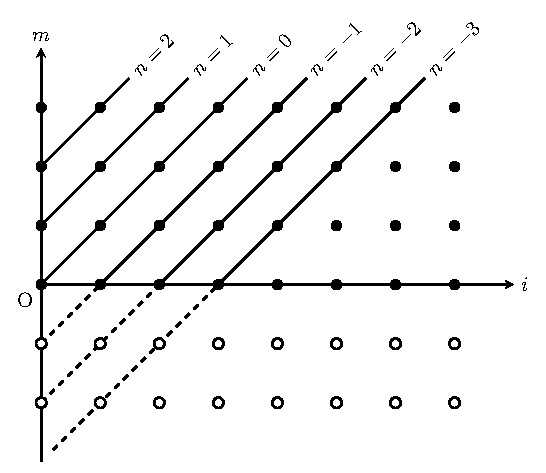
\includegraphics[width=58mm]{../TikZ/bessel/bessel.pdf}
    \caption{二重和の取りかえ方}
    \label{fig:bessel}
 \end{minipage}
  \end{tabular}
\end{figure}

\vspace{-12pt}
\begin{equation*}
  g(t, x) = \sum_{n=-\infty}^\infty \sum_{i=0}^\infty \frac{(-1)^i}{i! \, (n+i)!} \( \frac{x}{2} \)^{n+2i} t^{n}
\end{equation*}
母関数\eqref{eq:Jn-gene}の右辺と比較して
\begin{equation*}
  J_n(x) = \sum_{i=0}^\infty \frac{(-1)^i}{i! (n+i)!} \( \frac{x}{2} \)^{n+2i}
\end{equation*}\qed


\paragraph{母関数 $\Longrightarrow$ 漸化式}
母関数\eqref{eq:Jn-gene}の中辺を$t$について偏微分することで
\begin{equation}\label{eq:Jn-gene->req}
  \frac{\6 g(t, x)}{\6 t} = \frac{x}{2} \( 1+\frac{1}{t^2} \) g(t, x)
\end{equation}
が成立することが分かる。いま、母関数\eqref{eq:Jn-gene}の右辺から
\begin{equation*}
  \frac{\6 g(t, x)}{\6 t} = \sum_{n=-\infty}^\infty n J_n(x) t^{n-1}
\end{equation*}
であるので、これと母関数\eqref{eq:Jn-gene}の右辺を\eqref{eq:Jn-gene->req}に代入して
\begin{gather*}
  \sum_{n=-\infty}^\infty n J_n(x) t^{n-1}
	= \frac{x}{2} \( 1+\frac{1}{t^2} \) \sum_{n=-\infty}^\infty J_n(x) t^n\\
  \begin{split} \therefore
    \sum_{n=-\infty}^\infty \frac{2n}{x} J_n(x) t^{n-1}
	&= \sum_{n=-\infty}^\infty J_n(x) t^n 
			+ \sum_{n=-\infty}^\infty J_n(x) t^{n-2} \\
	&= \sum_{n=-\infty}^\infty \[ J_{n-1}(x) +  J_{n+1}(x) \]  t^{n-1}
  \end{split}
\end{gather*}
$t^{n-1}$の係数を比較して次を得る。
\begin{equation*}
  \frac{2n}{x} J_n(x) = J_{n-1} (x) + J_{n+1}(x)
\end{equation*}\qed


\paragraph{母関数 $\Longrightarrow$ 微分漸化式}

母関数\eqref{eq:Jn-gene}の中辺を$x$について偏微分することで
\begin{equation}\label{eq:Jn-gene->diffreq}
  \frac{\6 g(t, x)}{\6 x} = \frac{1}{2} \( t-\frac{1}{t} \) g(t, x)
\end{equation}
が成立することが分かる。いま、母関数\eqref{eq:Jn-gene}の右辺から
\begin{equation*}
  \frac{\6 g(t, x)}{\6 x} = \sum_{n=-\infty}^\infty \frac{d J_n(x)}{dx} t^{n}
\end{equation*}
であるので、これと母関数\eqref{eq:Jn-gene}の右辺を\eqref{eq:Jn-gene->diffreq}に代入して
\begin{gather*}
  \sum_{n=-\infty}^\infty \frac{d J_n(x)}{dx} t^{n}
	= \frac{1}{2} \( t-\frac{1}{t} \) \sum_{n=-\infty}^\infty J_n(x) t^n\\
  \begin{split}
    \sum_{n=-\infty}^\infty 2 \frac{d J_n(x)}{dx} t^{n}
	&= \sum_{n=-\infty}^\infty J_n(x) t^{n+1} 
		- \sum_{n=-\infty}^\infty J_n(x) t^{n-1} \notag\\
	&= \sum_{n=-\infty}^\infty \[ J_{n-1}(x) - J_{n+1} (x) \] t^n
  \end{split}
\end{gather*}
$t^{n}$の係数を比較して次を得る。
\begin{equation*}
  2 \frac{d J_n(x)}{dx} = J_{n-1}(x) - J_{n+1} (x)
\end{equation*}\qed


\paragraph{母関数, 微分漸化式 $\Longrightarrow$ 昇降演算子}

まず下降演算子については$\frac{1}{2} \[ \eqref{eq:Jn-diffreq} + \eqref{eq:Jn-req} \]$を計算して
\begin{equation*}
   \( \dx{} + \frac{n}{x} \) J_n(x) = J_{n-1}(x)
\end{equation*}
上昇演算子については$\frac{1}{2} \[ \eqref{eq:Jn-diffreq} - \eqref{eq:Jn-req} \]$を計算して
\begin{equation*}
   \( \dx{} - \frac{n}{x} \) J_n(x) = - J_{n+1}(x)
\end{equation*}\qed

\paragraph{昇降演算子 $\Longrightarrow$ 微分方程式}

上昇演算子\eqref{eq:Jn-josho}の両辺に左から$\( \dx{} + \frac{n+1}{x} \)$を作用させると、
左辺は
\begin{align*}
  \( \dx{} + \frac{n+1}{x} \) \( \dx{} - \frac{n}{x} \) J_n(x)
	&= \[ \dx{} \( \dx{} - \frac{n}{x} \) + \frac{n+1}{x} \( \dx{} - \frac{n}{x} \) \] J_n(x) \notag\\
	&= \[ \( \dx{2} + \frac{n}{x^2} - \frac{n}{x} \dx{} \) 
			+ \( \frac{n+1}{x} \dx{} - \frac{n^2+n}{x^2} \)  \] J_n(x)\notag\\
	&= \( \dx{2} + \frac{1}{x} \dx{} - \frac{n^2}{x^2} \) J_n(x)
\end{align*}
一方右辺は$- \( \dx{} + \frac{n+1}{x} \) J_{n+1}$であるがこれは下降演算子\eqref{eq:Jn-kako}から
$-J_n(x)$に等しい。よって、
\begin{equation*}
  \( \dx{2} + \frac{1}{x} \dx{} - \frac{n^2}{x^2} \) J_n(x) = -J_n(x) \qquad \therefore
	\frac{d^2 J_n(x)}{dx^2} + \frac{1}{x} \frac{d J_n(x)}{dx} + \( 1-\frac{n^2}{x^2} \) J_n(x) = 0
\end{equation*}
また、得られた微分方程式において$x\to kx$と置き換えると
\begin{gather*}
  \frac{d^2 J_n(kx)}{d(kx)^2} + \frac{1}{kx} \frac{d J_n(kx)}{d(kx)} + \( 1-\frac{n^2}{(kx)^2} \) J_n(kx) = 0
\end{gather*}
となり、
$\frac{d}{d(kx)} = \frac{dx}{d(kx)} \dx{} = \frac{1}{d(kx)/dx} \dx{} = \frac{1}{k} \dx{}$
に注意して整理すると\eqref{eq:Jn-diff-eq2}が得られる。
さらに\eqref{eq:Jn-diff-eq1}, \eqref{eq:Jn-diff-eq2}はそれぞれ\eqref{eq:Jn-self-1}, \eqref{eq:Jn-self-2}
のようにも書ける。
\qed

\vspace{10pt}
\paragraph{昇降演算子 $\Longrightarrow$ 微分・積分公式}

下降演算子\eqref{eq:Jn-kako}の両辺に$x^n$をかけると

\begin{equation*}
  \( x^n \dx{} + n x^{n-1} \) J_n(x) = x^n J_{n-1}(x) \qquad \therefore
	\dx{} [x^n J_n(x)] = x^n J_{n-1} (x)
\end{equation*}
これより積分公式は
\begin{equation*}
  \int x^n J_{n-1} (x) dx = x^n J_n(x) + C
\end{equation*}
同様に上昇演算子\eqref{eq:Jn-josho}の両辺に$x^{-n}$をかけると
\begin{equation*}
  \( x^{-n} \dx{} - nx^{-n-1} \) J_n(x) = - x^{-n} J_{n+1}(x) \qquad \therefore
	\dx{} [x^{-n} J_n(x)] = -x^{-n} J_{n+1} (x) 
\end{equation*}
これより積分公式は
\begin{equation*}
  \qquad \int x^{-n} J_{n+1} (x) dx = - x^{-n} J_n(x) + C
\end{equation*}\qed



%%%%%%%%%%%%%%%%%%%%%%%%%%%%%%%%%%%%%%%%%%%%%%%%%%%%

\subsection{一般次数のBessel関数(第1種Bessel関数)}

整数次のBessel関数$J_n(x)$は、一般項\eqref{eq:Jn-ippan}において整数$n$を
任意の実数$\nu$に置き換えることで一般次数まで拡張できる。
これに伴い階乗$(n+i)!$はガンマ関数$\Gamma(\nu+i+1)$に拡張される。
次数$\nu$が整数でないときは母関数は定義できない。
$J_\nu(x)$の定義域は複素数までカバーできるが、
\textbf{$\nu$が整数でないときは$J_\nu(x)$は負の実数上で定義されない}ことに注意が必要である
\footnote{指数関数$a^x$は$x\in\mathbb{Z}$を除いて$a<0$の領域で意味をなさない。}。
また、後で球Bessel関数についての重要な公式を導くために必要となる
高階導関数表示もここで紹介する。
これは$J_\nu(x)$に関する微分公式を$n$回用いるだけで導かれる。

\subsubsection*{公式集}

\vspace{12pt}
\paragraph{一般項(定義)}
\begin{equation}\label{eq:Jnu-ippan}
  J_\nu(x) = \sum_{i=0}^\infty \frac{(-1)^i}{i!\ \Gamma(\nu +i+1)} \( \frac{x}{2} \)^{\nu+2i}
	\quad (\nu \notin\mathbb{Z} \land x<0 を除く)
\end{equation}

\paragraph{漸化式}
\begin{equation}\label{eq:Jnu-req}
  \frac{2\nu}{x} J_{\nu}(x) = J_{\nu -1} (x) + J_{\nu +1}(x)
\end{equation}

\paragraph{微分漸化式}
\begin{equation}\label{eq:Jnu-diff-req}
  2\frac{d J_\nu (x)}{dx} = J_{\nu -1}(x) - J_{\nu +1} (x)
\end{equation}

\paragraph{昇降演算子}
\begin{alignat}{2}
  &\mathrm{\textbf{下降演算子}} & \quad & \( \dx{} + \frac{\nu}{x} \) J_\nu (x) = J_{\nu -1}(x) 
		\label{eq:Jnu-kako}\\
  &\mathrm{\textbf{上昇演算子}} &  & \( \dx{} - \frac{\nu}{x} \) J_\nu (x) =  - J_{\nu +1}(x) 
		\label{eq:Jnu-josho}
\end{alignat}

\paragraph{微分方程式}
\begin{gather}
  \frac{d^2 J_\nu (x)}{dx^2} + \frac{1}{x} \frac{d J_\nu (x)}{dx} + \( 1-\frac{\nu^2}{x^2} \) J_\nu (x) = 0 
	\label{eq:Jnu-diff-eq} \\
  \frac{d^2 J_\nu (kx)}{dx^2} + \frac{1}{x} \frac{d J_\nu (kx)}{dx} + \( k^2 -\frac{\nu^2}{x^2} \) J_\nu(kx) = 0
\end{gather}

\paragraph{自己随伴形}
\begin{gather}
  \dx{} \[ x \dx{} J_\nu (x) \] + \( x - \frac{\nu^2}{x} \) J_\nu (x) = 0 \label{eq:Jnu-self-1}\\
  \dx{} \[ x \dx{} J_\nu (kx) \] + \( k^2 x - \frac{\nu^2}{x} \) J_\nu (kx) = 0 \label{eq:Jnu-self-2}
\end{gather}

\paragraph{微分・積分公式}
\begin{alignat}{2}
  \dx{} [x^\nu J_\nu(x)] &= x^\nu J_{\nu-1}(x) , 
		&  \int x^\nu J_{\nu-1}(x) dx &= x^\nu J_\nu(x) + C 
		\label{eq:Jnu-bibun-1} \\
  \dx{} [x^{-\nu} J_\nu(x)] &= -x^{-\nu} J_{\nu+1} (x) , 
		&\quad\qquad \int x^{-\nu} J_{\nu+1} (x) dx &= - x^{-\nu} J_\nu(x) + C
		\label{eq:Jnu-bibun-2}
\end{alignat}

\paragraph{高階導関数表示}
$n=0, 1, 2, \dots$とすると
\begin{align}
  x^{-\nu-n} J_{\nu+n} (x) &= (-1)^n \( \frac{1}{x} \dx{} \)^n \[ x^{-\nu} J_\nu(x) \] \label{eq:Jnu-kokai-1}\\
  x^{\nu-n} J_{\nu-n} (x) &= \( \frac{1}{x} \dx{} \)^n \[ x^\nu J_\nu(x) \] \label{eq:Jnu-kokai-2}
\end{align}


% 図
\begin{figure}[tb]
\begin{tabular}{cc}
\hspace{-24pt}
 \begin{minipage}{0.50\hsize}\small
    \begin{figure}[H]
      \centering
      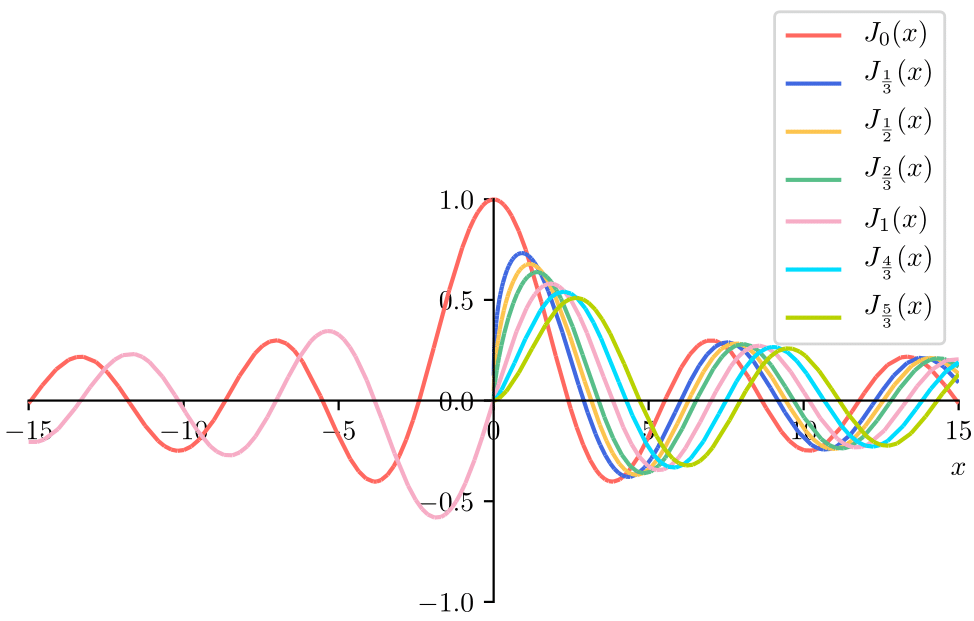
\includegraphics[width=75mm]{../fig/bessel/bessel_nu.png}
    \end{figure}
 \end{minipage}

 \begin{minipage}{0.50\hsize}
    \begin{figure}[H]
      \centering
      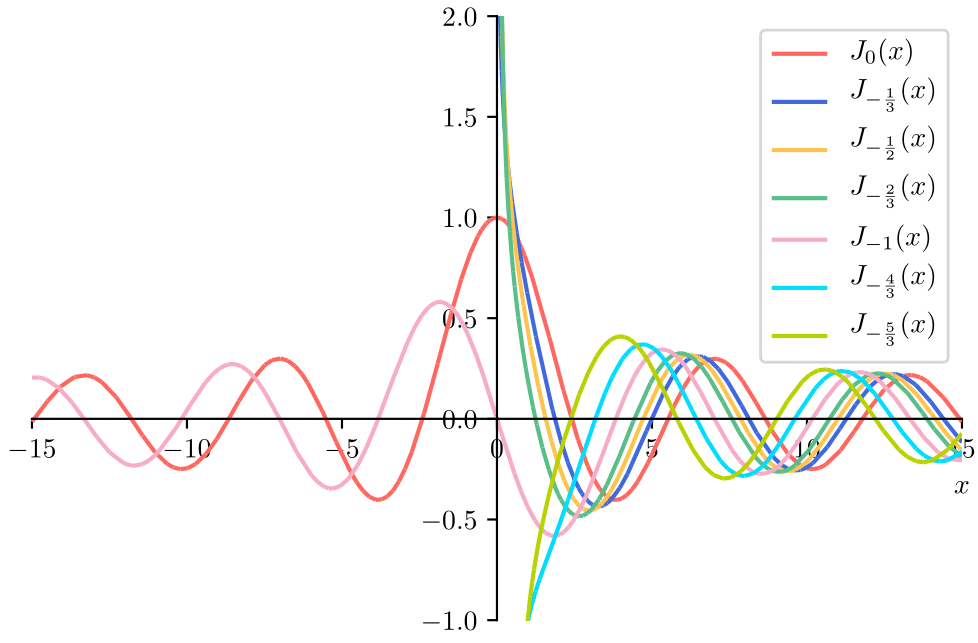
\includegraphics[width=75mm]{../fig/bessel/bessel_nu_minus.png}
    \end{figure}
 \end{minipage}
\end{tabular}
\caption{	一般次数のBessel関数 $J_\nu(x)$}
\end{figure}




\subsubsection*{証明}

一般項\eqref{eq:Jnu-ippan}が整数次のときと同形の
漸化式\eqref{eq:Jnu-req}および微分漸化式\eqref{eq:Jnu-diff-req}を満たすことを確認すれば、
後の昇降演算子や微分方程式、微分・積分公式は整数次のときとまったく同じ議論により
自動的に証明される。
最後の高階導関数表示だけは微分公式\eqref{eq:Jnu-bibun-1}, \eqref{eq:Jnu-bibun-2}から導く。

\paragraph{一般項 $\Longrightarrow$ 漸化式}

一般項\eqref{eq:Jnu-ippan}を用いて$J_{\nu -1} (x) + J_{\nu +1}(x)$を計算する。
\begin{align*}
  &\hspace{-24pt} J_{\nu -1} (x) + J_{\nu +1}(x) \notag\\
	&= \sum_{i=0}^\infty \frac{(-1)^i}{i!\ \Gamma(\nu +i)} \( \frac{x}{2} \)^{\nu+2i-1}
		+ \sum_{i=0}^\infty \frac{(-1)^i}{i!\ \Gamma(\nu +i+2)} \( \frac{x}{2} \)^{\nu+2i+1} \notag\\
	&= \[ \frac{1}{\Gamma(\nu)} \( \frac{x}{2} \)^{\nu-1}
			+ \sum_{i=1}^\infty \frac{(-1)^i}{i!\ \Gamma(\nu +i)} \( \frac{x}{2} \)^{\nu+2i-1} \]
		+ \sum_{i=1}^\infty \frac{(-1)^{i-1}}{(i-1)!\ \Gamma(\nu +i+1)} \( \frac{x}{2} \)^{\nu+2i-1} \notag\\
	&= \frac{1}{\Gamma(\nu)} \( \frac{x}{2} \)^{\nu-1}
		+ \sum_{i=1}^\infty \frac{(-1)^i}{i!\ \Gamma(\nu +i+1)} \( \frac{x}{2} \)^{\nu+2i-1}
			 [(\nu+i)-i] \notag\\
	&= \frac{1}{\Gamma(\nu)} \( \frac{x}{2} \)^{\nu-1}
		+ \sum_{i=1}^\infty \frac{(-1)^i \nu}{i!\ \Gamma(\nu +i+1)} \( \frac{x}{2} \)^{\nu+2i-1} \notag\\
	&= \sum_{i=0}^\infty \frac{(-1)^i \nu}{i!\ \Gamma(\nu +i+1)} \( \frac{x}{2} \)^{\nu+2i-1} 
		= \frac{2\nu}{x}
			\sum_{i=0}^\infty \frac{(-1)^i}{i!\ \Gamma(\nu +i+1)} \( \frac{x}{2} \)^{\nu+2i} \notag\\
	&= \frac{2\nu}{x} J_{\nu}(x) 
\end{align*}\qed

\paragraph{一般項 $\Longrightarrow$ 微分漸化式}

一般項\eqref{eq:Jnu-ippan}を用いて$2 \frac{d J_{\nu}(x)}{dx}$を計算する。
\begin{align*}
  2 \frac{d J_{\nu}(x)}{dx}
	&= 2 \dx{} \sum_{i=0}^\infty \frac{(-1)^i}{i!\ \Gamma(\nu +i+1)} \( \frac{x}{2} \)^{\nu+2i} \notag\\
	&= \sum_{i=0}^\infty \frac{(-1)^i (\nu+2i) }{i!\ \Gamma(\nu +i+1)} \( \frac{x}{2} \)^{\nu+2i-1} \notag\\
	&= \frac{\nu}{\Gamma (\nu+1)} \( \frac{x}{2} \)^{\nu-1}
		+ \sum_{i=1}^\infty \frac{(-1)^i (\nu+2i) }{i!\ \Gamma(\nu +i+1)} \( \frac{x}{2} \)^{\nu+2i-1} 
			\notag\\
	&= \frac{1}{\Gamma (\nu)} \( \frac{x}{2} \)^{\nu-1}
		+ \[ \sum_{i=1}^\infty \frac{(-1)^i (\nu+i) }{i!\ \Gamma(\nu +i+1)} \( \frac{x}{2} \)^{\nu+2i-1} 
			+ \sum_{i=1}^\infty \frac{(-1)^i i }{i!\ \Gamma(\nu +i+1)} \( \frac{x}{2} \)^{\nu+2i-1} \]
			\notag\\
	&= \[ \frac{1}{\Gamma (\nu)} \( \frac{x}{2} \)^{\nu-1}
			+ \sum_{i=1}^\infty \frac{(-1)^i}{i!\ \Gamma(\nu +i)} \( \frac{x}{2} \)^{\nu+2i-1} \]
		+ \sum_{i=1}^\infty \frac{(-1)^i}{(i-1)!\ \Gamma(\nu +i+1)} \( \frac{x}{2} \)^{\nu+2i-1} \notag\\
	&= \sum_{i=0}^\infty \frac{(-1)^i}{i!\ \Gamma(\nu +i)} \( \frac{x}{2} \)^{\nu+2i-1}
		-  \sum_{i=0}^\infty \frac{(-1)^i}{i!\ \Gamma(\nu +i+2)} \( \frac{x}{2} \)^{\nu+2i+1} \notag\\
	&= J_{\nu -1}(x) - J_{\nu +1} (x)
\end{align*}\qed


\paragraph{微分公式 $\Longrightarrow$ 高階導関数表示}
\eqref{eq:Jnu-bibun-2}の微分公式の両辺を$x$でわって
\begin{equation*}
  \frac{1}{x} \dx{} [x^{-\nu} J_\nu(x)] = -x^{-\nu-1} J_{\nu+1} (x)
\end{equation*}
と変形すると、関数$x^{-\nu} J_\nu(x)$に1回$\frac{1}{x} \dx{}$を作用させると
$x$の指数が1減り、Bessel関数の次数が1増え、符号が反転することが読み取れる。
したがって$x^{-\nu} J_\nu(x)$に対して$\frac{1}{x} \dx{}$を$n$回作用させると
\begin{equation*}
  \( \frac{1}{x} \dx{} \)^n [x^{-\nu} J_\nu(x)] = (-1)^n x^{-\nu-n} J_{\nu+n} (x)
\end{equation*}
となることが分かり、\eqref{eq:Jnu-kokai-1}が示される。
同様に\eqref{eq:Jnu-bibun-1}の微分公式の両辺を$x$でわって
\begin{equation*}
  \frac{1}{x} \dx{} [x^\nu J_\nu(x)] = x^{\nu-1} J_{\nu-1}(x)
\end{equation*}
と変形すると、関数$x^\nu J_\nu(x)$に1回$\frac{1}{x} \dx{}$を作用させると
$x$の指数とBessel関数の次数がともに1ずつ減ることが読み取れるので、
$x^\nu J_\nu(x)$に対して$\frac{1}{x} \dx{}$を$n$回作用させると
\begin{equation*}
  \( \frac{1}{x} \dx{} \)^n [x^\nu J_\nu(x)] = x^{\nu-n} J_{\nu-n}(x)
\end{equation*}
となることが分かり、\eqref{eq:Jnu-kokai-2}が示される。\qed


%%%%%%%%%%%%%%%%%%%%%%%%%%%%%%%%%%%%%%%%%%%%%%%%%%%%%%%%%%%%%%%%%%%%%%%
\subsection{Neumann関数(第2種Bessel関数)}

Besselの微分方程式\eqref{eq:Jnu-diff-eq}は2階であるので、
その基本解は$J_\nu(x)$のほかにもう1つあるはずである。
方程式中では$\nu$が$\nu^2$の形で現れているので、もうひとつの基本解としては
$J_{-\nu}(x)$が考えられ、
実際$\nu$が整数でないときは$J_\nu(x)$と$J_{-\nu}(x)$は線形独立となり基本解に選ぶことができる。
ところが$\nu$が整数$n$であるときは$J_n(x)$と$J_{-n}(x)$の間に\eqref{eq:Jn-fu}の関係があるため
線形独立とならず、基本解として選べない。
そこで$\nu$が整数であるときでもBesselの微分方程式\eqref{eq:Jnu-diff-eq}の2つ目の基本解を
構成できるものとして採用されるのが\eqref{eq:Nnu-def1}, \eqref{eq:Nnu-def2}により定義される
Neumann関数(第2種Bessel関数) $N_\nu(x)$である
\footnote{参考までに$J_\nu(x)$と$J_{-\nu}(x)$のロンスキアン $W[J_\nu, J_{-\nu}] (x)$、
$J_\nu(x)$と$N_\nu(x)$のロンスキアン $W[J_\nu, N_{\nu}] (x)$を記しておく。
\begin{align}
  &W[J_\nu, J_{-\nu}] (x) = J_\nu(x)J_{-\nu}^\prime(x)-J_\nu^\prime(x)J_{-\nu}(x) 
		= -\frac{2\sin\pi\nu}{\pi x} \\
  &W[J_\nu, N_{\nu}] (x) = J_\nu(x)N_{\nu}^\prime(x)-N_\nu^\prime(x)J_{\nu}(x) 
		= \frac{2}{\pi\nu}
\end{align}
}
。
$N_\nu(x)$は以下に示すように$J_\nu(x)$とまったく同形の漸化式、微分漸化式、昇降演算子、微分方程式、
微分・積分公式、高階導関数表示が成立する。



\subsubsection*{公式集}

\vspace{12pt}
\paragraph{定義}
\begin{alignat}{2}
  &N_\nu (x) = \frac{J_\nu (x) \cos\pi\nu - J_{-\nu}(x) }{ \sin\pi\nu} &\qquad & (\nu \notin \mathbb{Z})
	\label{eq:Nnu-def1}\\
  &N_n (x) = \lim_{\nu\to n} N_\nu (x) & & (\nu = n \in \mathbb{Z})
	\label{eq:Nnu-def2}
\end{alignat}

\paragraph{整数次の表式}
\begin{equation}\label{eq:Nn-hyo}
  N_n (x) = \frac{1}{\pi} \[ \frac{\6 J_\nu (x)}{\6 \nu} - (-1)^n  \frac{\6 J_{-\nu} (x)}{\6 \nu} \]_{\nu =n}
\end{equation}

\paragraph{非負整数次の一般項(参考)}\hspace{-12pt}\footnote{
ここで$\psi(z)$はディガンマ関数と呼ばれ、次のように定義される。
\begin{equation}
  \psi(z) = \dx{} \log \Gamma(z) = \frac{\Gamma^\prime (z)}{\Gamma (z)}
\end{equation}
}
\begin{align}
  N_n(x) &= \frac{2}{\pi} J_n(x) \log \frac{x}{2} \notag\\
	&\hspace{24pt} - \frac{1}{\pi} \sum_{i=0}^\infty \frac{(-1)^i}{i! (n+i)!} \( \frac{x}{2} \)^{n+2i}
		\[ \psi (i+1) + \psi(n+i+1) \] \notag\\
	&\hspace{24pt} -\frac{1}{\pi} \sum_{i=0}^{n-1} \frac{(n-i-1)!}{i!} \( \frac{x}{2} \)^{-n+2i}
		\qquad (n= 0, 1, 2, \dots)
\end{align}

% 後はEuler定数とか使います?

\paragraph{負の整数次}
\begin{equation}\label{eq:Nn-minus}
  N_{-n} (x) = (-1)^n N_n(x)
\end{equation}

\paragraph{漸化式}
\begin{equation}\label{eq:Nnu-req}
  \frac{2\nu}{x} N_{\nu}(x) = N_{\nu -1} (x) + N_{\nu +1}(x)
\end{equation}

\paragraph{微分漸化式}
\begin{equation}\label{eq:Nnu-req-diff}
  2\frac{d N_\nu (x)}{dx} = N_{\nu -1}(x) - N_{\nu +1} (x)
\end{equation}

\paragraph{昇降演算子}
\begin{alignat}{2}
  &\mathrm{\textbf{下降演算子}} & \quad & \( \dx{} + \frac{\nu}{x} \) N_\nu (x) = N_{\nu -1}(x) \\
  &\mathrm{\textbf{上昇演算子}} &  & \( \dx{} - \frac{\nu}{x} \) N_\nu (x) =  - N_{\nu +1}(x) 
\end{alignat}

\paragraph{微分方程式}
\begin{gather}
  \frac{d^2 N_\nu (x)}{dx^2} + \frac{1}{x} \frac{d N_\nu (x)}{dx} + \( 1-\frac{\nu^2}{x^2} \) N_\nu (x) = 0 
		\label{eq:Nnu-diff-eq}\\
  \frac{d^2 N_\nu (kx)}{dx^2} + \frac{1}{x} \frac{d N_\nu (kx)}{dx} + \( k^2 -\frac{\nu^2}{x^2} \) N_\nu(kx) = 0
\end{gather}


\paragraph{自己随伴形}
\begin{gather}
  \dx{} \[ x \dx{} N_\nu (x) \] + \( x - \frac{\nu^2}{x} \) N_\nu (x) = 0 \\
  \dx{} \[ x \dx{} N_\nu (kx) \] + \( k^2 x - \frac{\nu^2}{x} \) N_\nu (kx) = 0 
\end{gather}

\paragraph{微分・積分公式}
\begin{alignat}{2}
  \dx{} [x^\nu N_\nu(x)] &= x^\nu N_{\nu-1}(x) , 
		&  \int x^\nu N_{\nu-1}(x) dx &= x^\nu N_\nu(x) + C \\
  \dx{} [x^{-\nu} N_\nu(x)] &= -x^{-\nu} N_{\nu+1} (x) , 
		&\quad\qquad \int x^{-\nu} N_{\nu+1} (x) dx &= - x^{-\nu} N_\nu(x) + C
\end{alignat}

\paragraph{高階導関数表示}
$n=0, 1, 2, \dots$とすると
\begin{align}
  x^{-\nu-n} N_{\nu+n} (x) &= (-1)^n \( \frac{1}{x} \dx{} \)^n \[ x^{-\nu} N_\nu(x) \] \\
  x^{\nu-n} N_{\nu-n} (x) &= \( \frac{1}{x} \dx{} \)^n \[ x^\nu N_\nu(x) \] \label{eq:Nnu-kokai}
\end{align}


% 図
\begin{figure}[tb]
\begin{tabular}{cc}
\hspace{-24pt}
 \begin{minipage}{0.50\hsize}\small
    \begin{figure}[H]
      \centering
      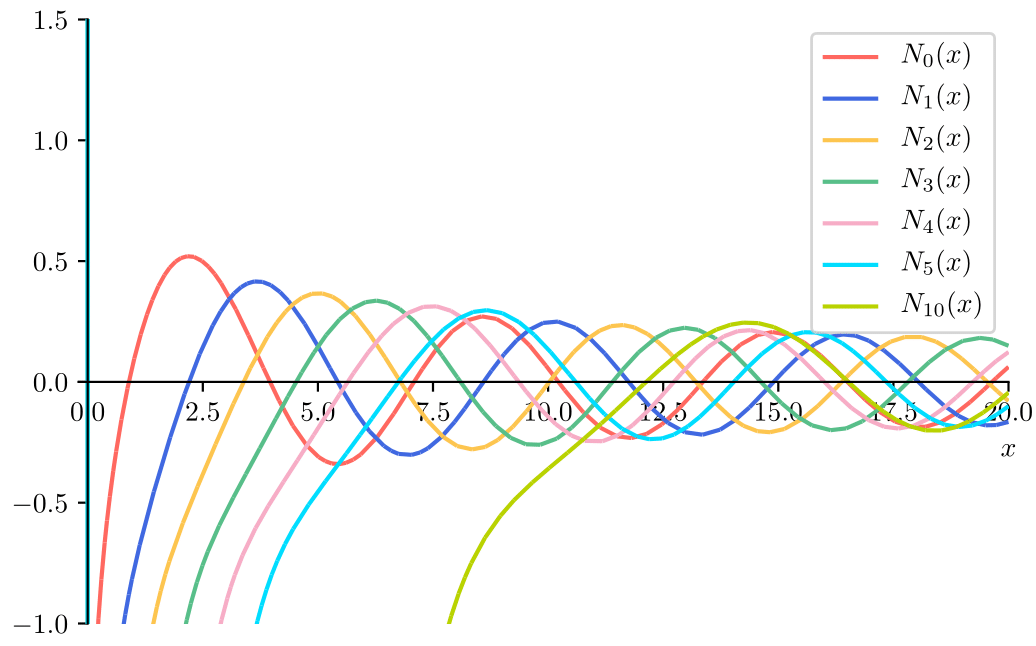
\includegraphics[width=75mm]{../fig/bessel/neumann_n.png}
    \end{figure}
 \end{minipage}

 \begin{minipage}{0.50\hsize}
    \begin{figure}[H]
      \centering
      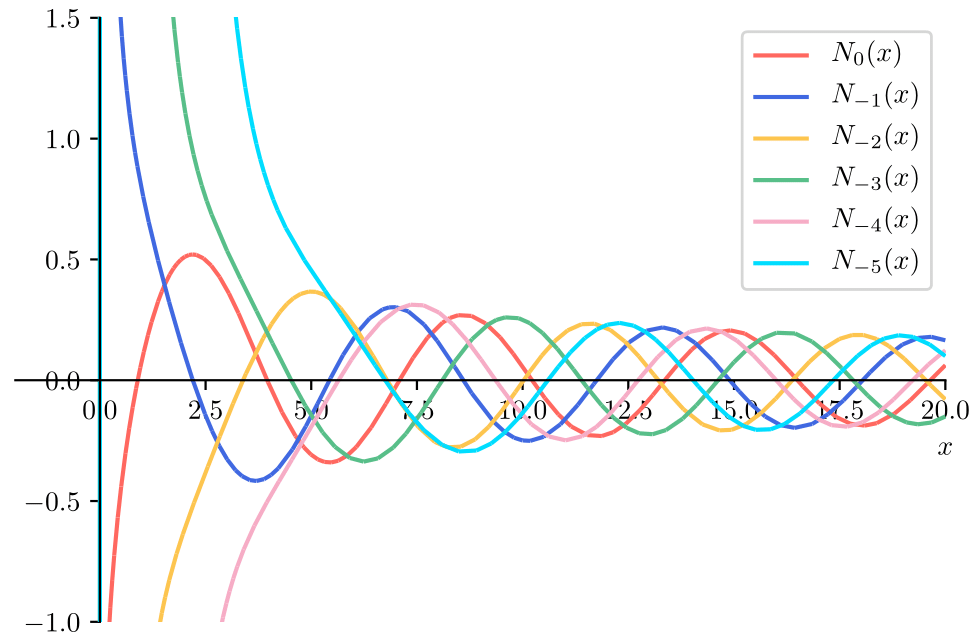
\includegraphics[width=75mm]{../fig/bessel/neumann_n_minus.png}
    \end{figure}
 \end{minipage}
\end{tabular}

\begin{tabular}{cc}
\hspace{-22pt}
 \begin{minipage}{0.50\hsize}
    \begin{figure}[H]
      \centering
      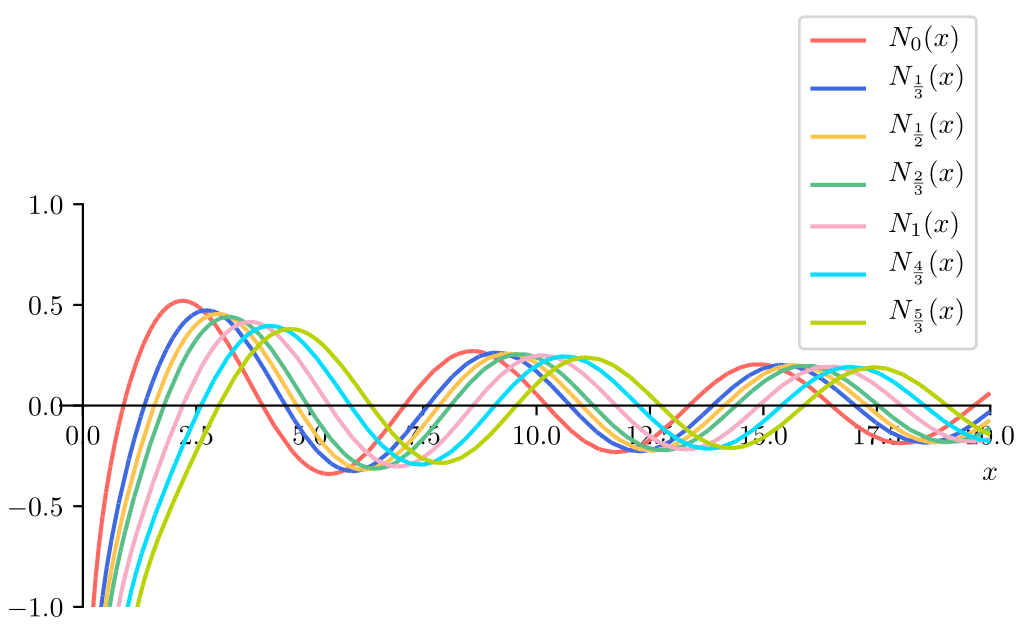
\includegraphics[width=75mm]{../fig/bessel/neumann_nu.png}
    \end{figure}
 \end{minipage}

 \hspace{1pt}
 \begin{minipage}{0.50\hsize}
    \begin{figure}[H]
      \centering
      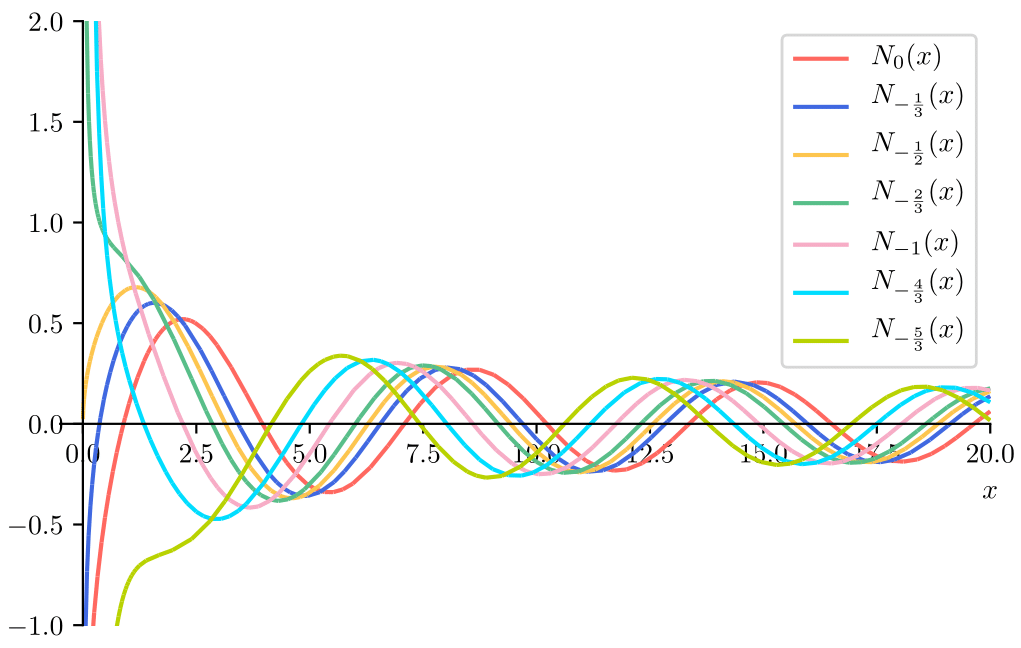
\includegraphics[width=75mm]{../fig/bessel/neumann_nu_minus.png}
    \end{figure}
 \end{minipage}
\end{tabular}
\caption{Neumann関数 $N_\nu(x)$}
\end{figure}


\subsubsection*{証明}
まず定義\eqref{eq:Nnu-def1}, \eqref{eq:Nnu-def2}から整数次についての等式
\eqref{eq:Nn-hyo}~\eqref{eq:Nn-minus}を示す。
次に定義\eqref{eq:Nnu-def1}と整数次の表式\eqref{eq:Nn-hyo}から
$J_\nu(x)$と同じ漸化式\eqref{eq:Nnu-req}および微分漸化式\eqref{eq:Nnu-req-diff}が
成り立つことを確認する。
すると残りの\eqref{eq:Nnu-diff-eq}~\eqref{eq:Nnu-kokai}はすべて
$J_n(x), J_\nu(x)$のときとまったく同じ議論により自動的に証明される。


\vspace{10pt}
\paragraph{定義 $\Longrightarrow$ 整数次の表式}

極限\eqref{eq:Nnu-def2}は$\frac{0}{0}$不定形であるので
L'H\^opitalの定理を用いることができる。
\begin{align*}
  N_n(x) 
	&= \lim_{\nu\to n} \frac{J_\nu (x) \cos\pi\nu - J_{-\nu}(x) }{ \sin\pi\nu} \notag\\
	&= \lim_{\nu\to n} 
		\frac{\frac{\6 J_\nu(x)}{\6\nu} \cos\pi\nu - J_\nu(x)\pi\sin\pi\nu -\frac{\6 J_{\nu}(x)}{\6\nu}}
				 {\pi\cos\pi\nu} \notag\\
	&= \frac{1}{\pi} \[ \frac{\6 J_\nu(x)}{\6\nu} - (-1)^n \frac{\6 J_{-\nu}(x)}{\6 \nu} \]_{\nu=n}
\end{align*}\qed

\paragraph{整数次の表式 $\Longrightarrow$ 負の整数次}

整数次の表式\eqref{eq:Nn-hyo}から
\begin{align*}
  N_{-n} (x) 
	&= \frac{1}{\pi} \[ \frac{\6 J_\nu (x)}{\6 \nu} 
		- (-1)^{-n}  \frac{\6 J_{-\nu} (x)}{\6 \nu} \]_{\nu =-n} \notag\\
	&= \frac{1}{\pi} \[ \frac{\6 J_{-\nu} (x)}{\6 (-\nu)} 
		- (-1)^{n}  \frac{\6 J_{\nu} (x)}{\6 (-\nu)} \]_{\nu =n} \notag\\
	&= (-1)^n \frac{1}{\pi} \[ \frac{\6 J_\nu (x)}{\6 \nu} 
		- (-1)^{n}  \frac{\6 J_{-\nu} (x)}{\6 \nu} \]_{\nu =n} \notag\\
	&= (-1)^n N_{n} (x) \notag
\end{align*}\qed


\paragraph{定義, 整数次の表式 $\Longrightarrow$ 漸化式}
$\nu \notin\mathbb{Z}$のとき、\eqref{eq:Nnu-def1}から
\begin{align*}
  &\hspace{-24pt}N_{\nu-1}(x) + N_{\nu+1}(x) \notag\\
	&= \frac{J_{\nu -1} (x) \cos\pi(\nu-1) - J_{-\nu+1}(x) }{ \sin\pi (\nu -1)}
		+ \frac{J_{\nu +1} (x) \cos\pi (\nu+1) - J_{-\nu-1}(x) }{ \sin\pi (\nu +1)} \notag\\
	&= \frac{J_{\nu-1} (x) \cos\pi\nu + J_{-\nu+1}(x) }{ \sin\pi\nu}
		+ \frac{J_{\nu +1} (x) \cos\pi\nu + J_{-\nu -1}(x) }{ \sin\pi\nu} \notag\\
	&= \frac{(J_{\nu -1}(x) + J_{\nu +1}(x))\cos\pi\nu + (J_{-\nu -1}(x) + J_{-\nu +1}(x))}
			{\sin\pi\nu} \notag\\
	&= \frac{2\nu}{x} \frac{J_\nu (x)\cos\pi\nu -J_{-\nu}(x)}{\sin\pi\nu}	
		\qquad (\eqref{eq:Jnu-req}を用いた) \notag\\
	&= \frac{2\nu}{x} N_\nu (x)
\end{align*}
次に$\nu=n \in\mathbb{Z}$のとき、\eqref{eq:Nn-hyo}から
\begin{align*}
  &\hspace{-24pt}N_{n-1}(x) + N_{n+1}(x) \notag\\
	&= \frac{1}{\pi} \[ \frac{\6 J_\nu (x)}{\6 \nu} - (-1)^{n-1}  \frac{\6 J_{-\nu} (x)}{\6 \nu} \]_{\nu =n-1}
		+ \frac{1}{\pi} \[ \frac{\6 J_\nu (x)}{\6 \nu} 
			- (-1)^{n+1} \frac{\6 J_{-\nu} (x)}{\6 \nu} \]_{\nu =n+1} \notag\\
	&= \frac{1}{\pi} \[  \frac{\6 J_{\nu-1} (x)}{\6 \nu} - (-1)^{n-1}  \frac{\6 J_{-\nu+1} (x)}{\6 \nu}
		+ \frac{\6 J_{\nu+1} (x)}{\6 \nu} - (-1)^{n+1} \frac{\6 J_{-\nu-1} (x)}{\6 \nu} \]_{\nu=n}\notag\\
	&= \frac{1}{\pi} \[ \frac{\6}{\6\nu}\( J_{\nu-1}(x) + J_{\nu+1}(x) \)
		+ (-1)^n \frac{\6}{\6 \nu} \( J_{-\nu-1}(x) + J_{-\nu+1}(x) \) \]_{\nu=n}\notag\\
	&= \frac{1}{\pi} \[ \frac{\6}{\6 \nu} \( \frac{2\nu}{x} J_\nu (x) \)
		+ (-1)^n \frac{\6}{\6\nu} \( \frac{-2\nu}{x} J_{-\nu} (x) \) \]_{\nu=n}\notag\\
	&= \frac{1}{\pi} \[ \frac{2}{x} J_\nu (x) + \frac{2\nu}{x} \frac{\6 J_\nu(x)}{\6 \nu}
		-(-1)^n \left\{ \frac{2}{x} J_{-\nu}(x) + \frac{2\nu}{x} \frac{\6 J_{-\nu}(x)}{\6\nu} \right\} \]_{\nu=n}
		\notag\\
	&= \frac{2n}{x} \cdot
		\frac{1}{\pi} \[ \frac{\6 J_\nu (x)}{\6 \nu} 
		- (-1)^n \frac{\6 J_{-\nu} (x)}{\6 \nu} \]_{\nu =n} \qquad (J_{-n}(x) = (-1)^nJ_n(x)を用いた)\notag\\
	&= \frac{2n}{x} N_n(x)
\end{align*}\qed


\paragraph{定義, 整数次の表式 $\Longrightarrow$ 微分漸化式}
$\nu \notin\mathbb{Z}$のとき、\eqref{eq:Nnu-def1}から
\begin{align*}
  &\hspace{-24pt}N_{\nu-1}(x) - N_{\nu+1}(x) \notag\\
	&= \frac{J_{\nu -1} (x) \cos\pi(\nu-1) - J_{-\nu+1}(x) }{ \sin\pi (\nu -1)}
		- \frac{J_{\nu +1} (x) \cos\pi (\nu+1) - J_{-\nu-1}(x) }{ \sin\pi (\nu +1)} \notag\\
	&= \frac{J_{\nu-1} (x) \cos\pi\nu + J_{-\nu+1}(x) }{ \sin\pi\nu}
		- \frac{J_{\nu +1} (x) \cos\pi\nu + J_{-\nu -1}(x) }{ \sin\pi\nu} \notag\\
	&= \frac{(J_{\nu -1}(x) - J_{\nu +1}(x))\cos\pi\nu - (J_{-\nu -1}(x) - J_{-\nu +1}(x))}
			{\sin\pi\nu} \notag\\
	&= 2\dx{} \frac{J_\nu (x)\cos\pi\nu -J_{-\nu}(x)}{\sin\pi\nu}	
		\qquad (\eqref{eq:Jnu-diff-req}を用いた) \notag\\
	&= 2\frac{d N_\nu (x)}{dx}
\end{align*}

次に$\nu=n \in\mathbb{Z}$のとき、\eqref{eq:Nn-hyo}から
\begin{align*}
  &\hspace{-24pt}N_{n-1}(x) - N_{n+1}(x) \notag\\
	&= \frac{1}{\pi} \[ \frac{\6 J_\nu (x)}{\6 \nu} - (-1)^{n-1}  \frac{\6 J_{-\nu} (x)}{\6 \nu} \]_{\nu =n-1}
		- \frac{1}{\pi} \[ \frac{\6 J_\nu (x)}{\6 \nu} 
			-(-1)^{n+1} \frac{\6 J_{-\nu} (x)}{\6 \nu} \]_{\nu =n+1} \notag\\
	&= \frac{1}{\pi} \[  \frac{\6 J_{\nu-1} (x)}{\6 \nu} - (-1)^{n-1}  \frac{\6 J_{-\nu+1} (x)}{\6 \nu}
		- \frac{\6 J_{\nu+1} (x)}{\6 \nu} + (-1)^{n+1} \frac{\6 J_{-\nu-1} (x)}{\6 \nu} \]_{\nu=n}\notag\\
	&= \frac{1}{\pi} \[ \frac{\6}{\6\nu}\( J_{\nu-1}(x) - J_{\nu+1}(x) \)
		- (-1)^n \frac{\6}{\6 \nu} \( J_{-\nu-1}(x) - J_{-\nu+1}(x) \) \]_{\nu=n}\notag\\
	&= \frac{1}{\pi} \[ \frac{\6}{\6 \nu} \( 2\frac{d J_\nu (x)}{dx} \)
		- (-1)^n \frac{\6}{\6\nu} \( 2\frac{ J_{-\nu} (x)}{dx} \) \]_{\nu=n}\notag\\
	&= 2\frac{d}{dx} \cdot
		\frac{1}{\pi} \[ \frac{\6 J_\nu (x)}{\6 \nu} 
		- (-1)^n \frac{\6 J_{-\nu} (x)}{\6 \nu} \]_{\nu =n}\notag\\
	&= 2\frac{d N_n(x)}{dx}
\end{align*}\qed



%%%%%%%%%%%%%%%%%%%%%%%%%%%%%%%%%%%%%%%%%%%%%%%%%%
\subsection{Hankel関数(第3種Bessel関数)}
後述する漸近形の節で示すように、$x$が十分大きい領域では
$J_\nu(x)$は$\cos$、$N_\nu(x)$は$\sin$のように振舞うことが知られている。
これまで三角関数$\cos x, \sin x$の
代わりに指数関数$e^{\pm ix} = \cos x \pm i\sin x$を用いて議論すると、
計算などにおいて便利になる場面が幾度かあった。
同じように$J_\nu(x), N_\nu(x)$の代わりに$J_\nu (x) \pm i N_\nu (x)$を考えると便利になることがある。
このように定義される関数をHankel関数(第3種Bessel関数)という。
正のほうは第1種Hankel関数と呼ばれ、負のほうは第2種Hankel関数と呼ばれる。

\vspace{12pt}
\paragraph{定義}
\begin{alignat}{2}
  H_\nu^{(1)} (x) &= J_\nu (x) + i N_\nu (x) &\qquad& (第1種\mathrm{Hankel}関数) \\
  H_\nu^{(2)} (x) &= J_\nu (x) - i N_\nu (x) & & (第2種\mathrm{Hankel}関数)
\end{alignat}

\subsection{円柱関数まとめ}
$J_\nu(x), N_\nu(x), H_\nu^{(1)} (x), H_\nu^{(2)} (x)$を総称して円柱関数と呼ぶ。

\subsubsection{Besselの微分方程式の一般解}

Besselの微分方程式
\begin{equation}
  \frac{d^2 y}{dx^2} + \frac{1}{x} \frac{dy}{dx} + \( 1-\frac{\nu^2}{x^2} \)y = 0
\end{equation}
の一般解は、
\begin{enumerate}
  \item $\nu$が整数でないならば
  \begin{equation}
    y = c_1 J_\nu (x) + c_2 J_{-\nu} (x)
  \end{equation}
  \item 一般には
  \begin{equation}
    y = c_1 J_\nu (x) + c_2 N_\nu (x) \quad あるいは \quad
    y = c_1 H_\nu^{(1)} (x) + c_2 H_\nu^{(2)} (x) 
  \end{equation}
\end{enumerate}
と書ける。


\subsubsection{円柱関数の共通の性質}
任意の円柱関数$Z_\nu (x)$は以下を共通で満たす。

\paragraph{漸化式}
\begin{equation}\label{eq:Znu-req}
  \frac{2\nu}{x} Z_{\nu}(x) = Z_{\nu -1} (x) + Z_{\nu +1}(x)
\end{equation}

\paragraph{微分漸化式}
\begin{equation}\label{eq:Znu-req-diff}
  2\frac{d Z_\nu (x)}{dx} = Z_{\nu -1}(x) - Z_{\nu +1} (x)
\end{equation}

\paragraph{昇降演算子}
\begin{alignat}{2}
  &\mathrm{\textbf{下降演算子}} & \quad & \( \dx{} + \frac{\nu}{x} \) Z_\nu (x) = Z_{\nu -1}(x) \\
  &\mathrm{\textbf{上昇演算子}} &  & \( \dx{} - \frac{\nu}{x} \) Z_\nu (x) =  - Z_{\nu +1}(x) 
\end{alignat}

\paragraph{微分方程式}
\begin{gather}
  \frac{d^2 Z_\nu (x)}{dx^2} + \frac{1}{x} \frac{d Z_\nu (x)}{dx} + \( 1-\frac{\nu^2}{x^2} \) Z_\nu (x) = 0 \\
 \frac{d^2 Z_\nu (kx)}{dx^2} + \frac{1}{x} \frac{d Z_\nu (kx)}{dx} + \( k^2 -\frac{\nu^2}{x^2} \) Z_\nu(kx) = 0
  \label{eq:Znu-diff-2}
\end{gather}


\paragraph{自己随伴形}
\begin{gather}
  \dx{} \[ x \dx{} Z_\nu (x) \] + \( x - \frac{\nu^2}{x} \) Z_\nu (x) = 0 \\
  \dx{} \[ x \dx{} Z_\nu (kx) \] + \( k^2 x - \frac{\nu^2}{x} \) Z_\nu (kx) = 0 
\end{gather}

\paragraph{微分・積分公式}
\begin{alignat}{2}
  \dx{} [x^\nu Z_\nu(x)] &= x^\nu Z_{\nu-1}(x) , 
		&  \int x^\nu Z_{\nu-1}(x) dx &= x^\nu Z_\nu(x) + C \\
  \dx{} [x^{-\nu} Z_\nu(x)] &= -x^{-\nu} Z_{\nu+1} (x) , 
		&\quad\qquad \int x^{-\nu} Z_{\nu+1} (x) dx &= - x^{-\nu} Z_\nu(x) + C
\end{alignat}

\paragraph{高階導関数表示}
$n=0, 1, 2, \dots$とすると
\begin{align}
  x^{-\nu-n} Z_{\nu+n} (x) &= (-1)^n \( \frac{1}{x} \dx{} \)^n \[ x^{-\nu} Z_\nu(x) \] \\
  x^{\nu-n} Z_{\nu-n} (x) &= \( \frac{1}{x} \dx{} \)^n \[ x^\nu Z_\nu(x) \]
\end{align}




\subsection{漸近形(参考)}

\paragraph{漸近形}
十分大きな$x$に対して
\begin{align}
  J_\nu (x) &\sim \sqrt{\frac{2}{\pi x}} \cos \( x - \frac{\pi\nu}{2} - \frac{\pi}{4} \) \\
  N_\nu (x) &\sim \sqrt{\frac{2}{\pi x}} \sin \( x - \frac{\pi\nu}{2} - \frac{\pi}{4} \) \\
  H_\nu^{(1)} (x) &\sim \sqrt{\frac{2}{\pi x}} \exp \[ i \( x - \frac{\pi\nu}{2} - \frac{\pi}{4} \) \] \\
  H_\nu^{(2)} (x) &\sim \sqrt{\frac{2}{\pi x}} \exp \[ -i \( x - \frac{\pi\nu}{2} - \frac{\pi}{4} \) \]
\end{align}
すなわち、$J_\nu (x), N_\nu(x)$は$x$が大きい領域では振幅が$\sqrt{x}$に反比例して小さくなる三角関数のように
振舞う(図\ref{fig:Znu-zenkin}参照)。

\begin{figure}[t]
  \centering
  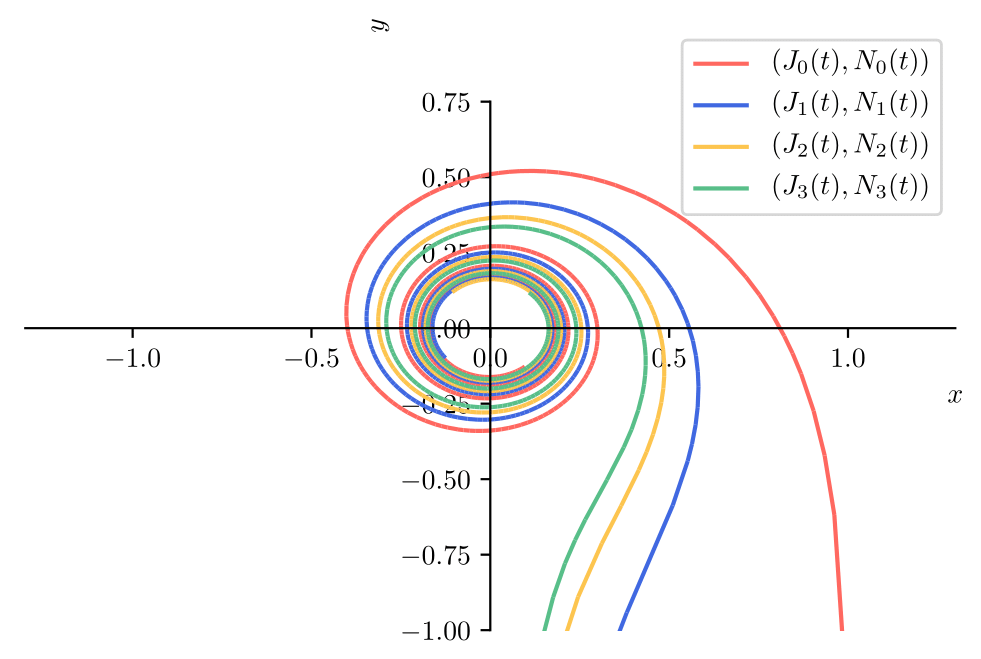
\includegraphics[width=80mm]{../fig/bessel/parametric-bessel.png}
  \caption{$(x, y)= (J_n (t), N_n (t)) \ (n=0, 1, 2, 3)$とした図。
	$t$が大きくなると半径を小さくしながら円に収束してゆく様子が分かる}
  \label{fig:Znu-zenkin}
\end{figure}

\subsection{Fourier-Bessel展開}
\subsubsection{Bessel関数の直交性}
Bessel関数は他の特殊関数と同様に直交性を持っている。
ただしBessel関数の直交性は少し趣が異なっており、
他の特殊関数のように異なる次数同士の関数の積を考えるのではなく、
同じ次数であるが引数が異なるもの同士の関数の積を考えることになる。
区間$[0, a]$に対する直交性を考えることができるが、
その際Bessel関数の零点と呼ばれるものが重要な役割を果たすことになる。

\begin{ibox}{Bessel関数の直交性}
一般次数のBessel関数$J_\nu(x) \ (\nu > -1)$について、
$J_\nu( \alpha ) = 0$を満たす正の数$\alpha$(Bessel関数の零点という)を小さい順に
$\alpha_{\nu 1}, \alpha_{\nu 2}, \dots$とすると、次の直交性が成立する。
\begin{equation}\label{eq:Jnu-choko}
  \int_0^a x \, J_\nu \(\frac{\alpha_{\nu m}}{a}x\) J_\nu \(\frac{\alpha_{\nu n}}{a}x \)dx
	= \frac{a^2}{2}\[ J_{\nu+1}(\alpha_{\nu n}) \]^2 \delta_{mn}
\end{equation}
\end{ibox}
\begin{proof}
  これまで直交性は母関数を積分することで証明をしてきたが、
  今回は一般次数に対するBessel関数の直交性を示すことになるので、
  母関数がそもそも存在せず、それゆえ別の方法を考えねばならない。
  このような時は自己随伴形の微分方程式\eqref{eq:Jnu-self-2}を用いる
\footnote{
実は他の特殊関数の直交性も、自己随伴形の微分方程式から以下で行う処理と同様に示すことができる。
ただしその方法では規格化の絶対値を導くことはできないので、
他の特殊関数の直交性では母関数の積分により証明する手法を採用している。\vspace{8pt}
}
\footnote{
以下の証明において困惑しがちな部分を先にここで指摘しておく。\\
まず第一に$\[ \frac{d f(x)}{dx} \]_{x=a} = \frac{df(a)}{da}$である。
$f(x)$を$x$で微分した式に$x=a$を代入したものと、
先に$f(x)$に$x=a$を代入して、その後$a$を1つの変数と見てそれで微分したものが等しくなることは
少し考えると分かると思う。\\
第二に$f^\prime (ax) = \frac{d f(ax)}{d(ax)} = \frac{1}{a} \frac{d f(ax)}{dx}$である。
$f^\prime (ax) = \frac{d f(ax)}{dx}$ではない。
元々$f^\prime (ax)$とは関数$f(x)$を$x$で微分した式に対して$x$を$ax$に置き換えるという意味であった。
すなわち$f^\prime (ax) = \[ \frac{d f(x)}{dx} \]_{x\to ax}$である。
}
。
  
  \vspace{6pt}
  \textbf{\underline{直交性}}\quad 
  \eqref{eq:Jnu-self-2}において$k$の代わりに$\frac{\alpha_{\nu m}}{a}, \frac{\alpha_{\nu n}}{a}$
  としたものを並べてみると、
  \begin{align}
    &\dx{} \[ x \dx{} J_\nu \(\frac{\alpha_{\nu m}}{a}x\) \] 
		+ \( \frac{\alpha_{\nu m}^2}{a^2} x - \frac{\nu^2}{x} \) 
		J_\nu \(\frac{\alpha_{\nu m}}{a}x\) = 0
		\label{eq:Jnu-choko-pro-1}\\
    &\dx{} \[ x \dx{} J_\nu \(\frac{\alpha_{\nu n}}{a}x\) \] 
		+ \( \frac{\alpha_{\nu n}^2}{a^2} x - \frac{\nu^2}{x} \) 
		J_\nu \(\frac{\alpha_{\nu n}}{a}x\) = 0
		\label{eq:Jnu-choko-pro-2}
  \end{align}
  ここで
  $J_\nu \(\frac{\alpha_{\nu n}}{a}x\) \times \eqref{eq:Jnu-choko-pro-1}
		- J_\nu \(\frac{\alpha_{\nu m}}{a}x\) \times \eqref{eq:Jnu-choko-pro-2} $
  を計算すると、
\begin{align}
  &\hspace{-30pt}
  J_\nu \(\frac{\alpha_{\nu n}}{a}x\) \dx{} \[ x \dx{} J_\nu \(\frac{\alpha_{\nu m}}{a}x\) \] 
		- J_\nu \(\frac{\alpha_{\nu m}}{a}x\) \dx{} \[ x \dx{} J_\nu \(\frac{\alpha_{\nu n}}{a}x\) \] 
	\notag\\
	&= \frac{\alpha_{\nu n}^2 - \alpha_{\nu m}^2}{a^2} \ x \, 
		J_\nu \(\frac{\alpha_{\nu m}}{a}x\)  J_\nu \(\frac{\alpha_{\nu n}}{a}x\) 
  \label{eq:Jnu-choko-mn}
\end{align}
\eqref{eq:Jnu-choko-mn}の両辺を$x$について$0$から$a$まで積分すると、左辺は部分積分により
\begin{align}
  &\hspace{-30pt}
  \int_0^a J_\nu \(\frac{\alpha_{\nu n}}{a}x\) \dx{} \[ x \dx{} J_\nu \(\frac{\alpha_{\nu m}}{a}x\) \] dx
	- \int_0^a J_\nu \(\frac{\alpha_{\nu m}}{a}x\) \dx{} \[ x \dx{} J_\nu \(\frac{\alpha_{\nu n}}{a}x\) \]dx
	\notag\\
  &= \[ J_\nu \(\frac{\alpha_{\nu n}}{a}x\) x \dx{} J_\nu \(\frac{\alpha_{\nu m}}{a}x\) \]_0^a
      - \cancel{\int_0^a \dx{} \[ J_\nu \(\frac{\alpha_{\nu n}}{a}x\) \] x 
		 \dx{} \[ J_\nu \(\frac{\alpha_{\nu m}}{a}x \) \] dx } \notag\\
  &\hspace{24pt}
	- \[ J_\nu \(\frac{\alpha_{\nu m}}{a}x\) x \dx{} J_\nu \(\frac{\alpha_{\nu n}}{a}x\) \]_0^a
      + \cancel{\int_0^a \dx{} \[ J_\nu \(\frac{\alpha_{\nu m}}{a}x\) \] x 
		 \dx{} \[ J_\nu \(\frac{\alpha_{\nu n}}{a}x \) \] dx } \notag\\
  &= J_\nu \(\alpha_{\nu n} \) a \frac{d}{da} J_\nu \(\alpha_{\nu m}\)
	-  J_\nu \(\alpha_{\nu m}\) a \frac{d}{da} J_\nu \(\alpha_{\nu n}\) \label{eq:Jnu-choko-zero} \\
  &= 0 \notag
\end{align}
となる
\footnote{
\eqref{eq:Jnu-choko-zero}を得る際に$[..]_0^a$の内部が$x=0$で$0$になることを
あたかも自明であるかのように計算しているが、実はこれは$\nu > -1$でなければいうことができない
(一般項\eqref{eq:Jnu-ippan}から$[..]_0^a$の内部が$x\sim 0$でどうなるか考えてみよ)。
これが公式\eqref{eq:Jnu-choko}を提示する際にさりげなく$\nu>-1$という条件を設けた所以である。
またこのことを考慮に入れると、Bessel関数$J_\nu(x)$と同じ微分方程式を持つはずである
Neumann関数$N_\nu(x)$が
直交性を持たないことも分かると思う。
}
。
一方\eqref{eq:Jnu-choko-mn}の右辺は
\begin{equation*}
  \frac{\alpha_{\nu n}^2 - \alpha_{\nu m}^2}{a^2} 
	\int_0^a x \, J_\nu \(\frac{\alpha_{\nu m}}{a}x\) J_\nu \(\frac{\alpha_{\nu n}}{a}x \)dx
\end{equation*}
であるので、$m\neq n$であるとき
\begin{equation}\label{eq:Jnu-choko-pr}
  \int_0^a x \, J_\nu \(\frac{\alpha_{\nu m}}{a}x\) J_\nu \(\frac{\alpha_{\nu n}}{a}x \)dx
	= 0
\end{equation}
であることが確証される。

\vspace{6pt}
\textbf{\underline{規格化}}\quad 
ところが$m=n$であるときは、上の結果をそのまま用いると\eqref{eq:Jnu-choko-mn}の積分結果が
$0=0$となってしまい、意味を持たなくなってしまう。
そこで左辺の積分については\eqref{eq:Jnu-choko-zero}まで戻って
$\alpha_{\nu m} = \alpha_{\nu n} + \epsilon$として計算し、
最後に$\epsilon \to 0$の極限を取ることを考えればよい。
Taylor展開により$\epsilon$の1次の項まであらわに書くことにすると、\eqref{eq:Jnu-choko-zero}は
\begin{align}
  &\hspace{-24pt}
  J_\nu \(\alpha_{\nu n} \) a \frac{d}{da} J_\nu \(\alpha_{\nu m}\)
	-  J_\nu \(\alpha_{\nu m}\) a \frac{d}{da} J_\nu \(\alpha_{\nu n}\) \notag\\
  &= \cancel{J_\nu \(\alpha_{\nu n} \) a \frac{d}{da} J_\nu \(\alpha_{\nu n} + \epsilon\)}
	-  J_\nu \(\alpha_{\nu n} + \epsilon\) a \frac{d}{da} J_\nu \(\alpha_{\nu n}\) \notag\\
  &= -a\[ \cancel{J_\nu(\alpha_{\nu n})} + \epsilon J_\nu^\prime (\alpha_{\nu n}) 
	+ \mathcal{O} (\epsilon^2) \]
	\cdot {\frac{\alpha_{\nu n}}{a}} \cdot J_\nu^\prime (\alpha_{\nu n}) \notag\\
  &= - \epsilon \alpha_{\nu n} \[ J_\nu^\prime (\alpha_{\nu n}) \]^2 + \mathcal{O} (\epsilon^2)
	\label{eq:Jnu-kikaku-left}
\end{align}
一方\eqref{eq:Jnu-choko-mn}の右辺は
\begin{align}
  &\hspace{-24pt}
  \frac{\alpha_{\nu n}^2 - \alpha_{\nu m}^2}{a^2} 
	\int_0^a x \, J_\nu \(\frac{\alpha_{\nu m}}{a}x\) J_\nu \(\frac{\alpha_{\nu n}}{a}x \)dx \notag\\
  &= \frac{\alpha_{\nu n}^2 - (\alpha_{\nu n} + \epsilon)^2}{a^2} 
	\int_0^a x \, J_\nu \(\frac{\alpha_{\nu n} + \epsilon}{a}x\) J_\nu \(\frac{\alpha_{\nu n}}{a}x \)dx
	\notag\\
  &= -\frac{\epsilon \, (2\alpha_{\nu n} + \epsilon)}{a^2}
	\int_0^a x \, J_\nu \(\frac{\alpha_{\nu n} + \epsilon}{a}x\) J_\nu \(\frac{\alpha_{\nu n}}{a}x \)dx
	\label{eq:Jnu-kikaku-right}
\end{align}
であるので、\eqref{eq:Jnu-kikaku-left}, \eqref{eq:Jnu-kikaku-right}から
\begin{equation*}
   (2\alpha_{\nu n} + \epsilon) 
		\int_0^a x \, J_\nu \(\frac{\alpha_{\nu n} + \epsilon}{a}x\) J_\nu \(\frac{\alpha_{\nu n}}{a}x \)dx
	= a^2 \, \alpha_{\nu n} \[ J_\nu^\prime (\alpha_{\nu n}) \]^2 + \mathcal{O} (\epsilon)
\end{equation*}
$\epsilon \to 0$とすると
\begin{equation*}
  \int_0^a x \[ J_\nu \(\frac{\alpha_{\nu n}}{a}x \)\]^2 dx
	= \frac{a^2}{2}\[ J_{\nu}^\prime (\alpha_{\nu n}) \]^2
\end{equation*}
最後に上昇演算子\eqref{eq:Jnu-josho}から
\begin{equation*}
  J_{\nu}^\prime (\alpha_{\nu n})
	= \frac{\nu}{\alpha_{\nu n}} J_\nu (\alpha_{\nu n}) - J_{\nu +1}(\alpha_{\nu n})
	= - J_{\nu +1}(\alpha_{\nu n})
\end{equation*}
であることを用いると、次が成り立つことが示される。
\begin{equation}\label{eq:Jnu-kikaku-pr}
  \int_0^a x \[ J_\nu \(\frac{\alpha_{\nu n}}{a}x \)\]^2 dx
	= \frac{a^2}{2}\[ J_{\nu+1} (\alpha_{\nu n}) \]^2
\end{equation}

\vspace{6pt}
\eqref{eq:Jnu-choko-pr}, \eqref{eq:Jnu-kikaku-pr}をまとめると\eqref{eq:Jnu-choko}のように書ける。

\end{proof}


\subsubsection{Fourier-Bessel展開}
周期$L$の複素指数関数$e^{i\frac{2n\pi}{L}x} \ (n = 0, \pm1, \pm2, \dots)$は次のような直交性を持っていた。
\begin{equation*}
  \int_0^{L} e^{-\frac{2m\pi}{L}x} e^{i\frac{2n\pi}{L}x} dx
	= L \, \delta_{mn}
\end{equation*}
この直交性(と完全性)から、
区間$[0, L]$においてしかるべき条件
\footnote{区分的に滑らか、かつ絶対可積分であること。}
を持つ関数$f(x)$は次のようにFourier級数展開できるのであった。
\begin{alignat*}{2}
  &\textbf{展開式} && f(x) = \sum_{n=-\infty}^\infty c_n e^{i\frac{2n\pi}{L}x}  \\
  &\textbf{展開係数} &\quad & c_n = \frac{1}{L} \int_0^L e^{-i\frac{2n\pi}{L}x} f(x) dx
\end{alignat*}
一般次数のBessel関数にも直交性\eqref{eq:Jnu-choko}があるので、
Fourier級数展開と同じようなことができる。
これを\textbf{Fourier-Bessel展開}と呼ぶことがある。
Fourier-Bessel展開は円型膜の振動を考えるときなどに応用される( 問題[4-2] )。

\begin{ibox}{Fourier-Bessel展開}
  \noindent
  一般次数のBessel関数$J_\nu(x) \ (\nu >-1)$の正の零点を小さい順に
  $\alpha_{\nu 1}, \alpha_{\nu 2}, \dots$とする。
  区間$[0, a]$で定義された関数$f(x)$がしかるべき条件を持つとき、
  関数$f(x)$は次のようにFourier-Bessel展開できる。
  \begin{alignat}{2}
  &\textbf{展開式} && f(x) = \sum_{n=1}^\infty c_{\nu n} \, J_\nu \( \frac{\alpha_{\nu n}}{a} x \)  \\
  &\textbf{展開係数} &\quad & c_{\nu n} = \frac{2}{a^2 \[ J_{\nu+1} (\alpha_{\nu n}) \]^2} 
		\int_0^a x f(x) J_\nu \( \frac{\alpha_{\nu n}}{a} x \) dx
\end{alignat}
\end{ibox}

\noindent
\textbf{[例]\ $x^{\nu} \ (\nu>-1)$のFourier-Bessel展開 } 

\begin{table}[H]
  \small
  \begin{tabular}{c}
    
    \begin{minipage}{0.75\hsize}
        簡単に手計算できる例として、区間$[0, 1]$における$x^{\nu} \ (\nu>-1)$のFourier-Bessel展開を考えよう。
	上の公式で$f(x) = x^\nu \ (\nu >-1), \ a=1$とすると、展開係数$c_{\nu n}$は
	$z = \alpha_{\nu n} x, \ dx = \frac{1}{\alpha_{\nu n}} dz$なる置換により
    \end{minipage}

    \begin{minipage}{0.03\hsize}
      \hspace{1pt}
    \end{minipage}

    \begin{minipage}{0.2\hsize}\small
      \begin{tabular}{c||ccc}
        \hline
        $x$ & $0$ & $\rightarrow$ & $1$\\ \hline 
        $z$ & $0$ & $\rightarrow$ & $\alpha_{\nu n}$\\ \hline 
      \end{tabular}
    \end{minipage}

  \end{tabular}
\end{table}

\vspace{-24pt}
\begin{alignat*}{2}
  c_{\nu n}
	&= \frac{2}{\[ J_{\nu+1} (\alpha_{\nu n}) \]^2} 
		\int_0^1 x^{\nu+1} J_\nu \( \alpha_{\nu n} x \) dx \notag\\
	&= \frac{2}{\[ J_{\nu+1} (\alpha_{\nu n}) \]^2} \cdot \frac{1}{{\alpha_{\nu n}}^{\nu+2}}
		\int_0^{\alpha_{\nu n}} z^{\nu+1} J_\nu ( z ) dz \notag\\
	&= \frac{2}{\[ J_{\nu+1} (\alpha_{\nu n}) \]^2} \cdot \frac{1}{{\alpha_{\nu n}}^{\nu+2}}
		\[ z^{\nu+1} J_{\nu+1} (z) \]_0^{\alpha_{\nu n}}	&\qquad &(\since 積分公式\eqref{eq:Jnu-bibun-1})
		\notag\\
	&= \frac{2}{\alpha_{\nu n} J_{\nu+1}(\alpha_{\nu n})} & & (\since \nu > -1)
\end{alignat*}
よって区間$[0, 1]$における$x^{\nu} \ (\nu>-1)$のFourier-Bessel展開は次のようになる。
\begin{equation*}
  x^\nu = \sum_{n=1}^\infty \frac{2}{\alpha_{\nu n} J_{\nu+1}(\alpha_{\nu n})} 
		\, J_\nu ( \alpha_{\nu n} x ) 
\end{equation*}




\section{変形Bessel関数}
\subsection{第1種変形Bessel関数}
第1種変形Bessel関数$I_\nu (x)$は\eqref{eq:Inu-def}のようにBessel関数$J_\nu(x)$を用いて定義する。
虚数単位$i$を用いているが、このように定義しても$I_\nu(x)$が$\mathbb{R} \to \mathbb{R}$を満たすことは
Bessel関数の一般項\eqref{eq:Jnu-ippan}から容易に分かる。
$I_\nu (x)$に関する公式は$J_\nu(x)$に関する公式で$x$を$ix$に置き換えることで直ちに導かれる。
なおここでは記さないが、一度整数次の$I_n(x)$の母関数を証明しておくと、通常のBessel関数のときと同様に
整数次の$I_n(x)$に関する関係式を示すことができ、
また一般項を示すと一般次数の$I_\nu(x)$に関する関係式を導くことができる。

\subsubsection*{公式集}

\paragraph{定義}
\begin{equation}\label{eq:Inu-def}
  I_\nu (x) = i^{-\nu} J_\nu (ix)
\end{equation}

\paragraph{母関数}
\begin{equation}\label{eq:Inu-gene}
  g(t, x) = e^{\frac{x}{2} \( t+\frac{1}{t} \)}
	= \sum_{n=-\infty}^\infty I_n (x) t^n
\end{equation}

\paragraph{偶奇性}
\begin{equation}
  I_{n} (-x) = (-1)^n I_n (x)
\end{equation}


\paragraph{負の整数次}
\begin{equation}
  I_{-n} (x) = I_n(x)
\end{equation}

\paragraph{一般項}
\begin{equation}
  I_\nu(x) = \sum_{i=0}^\infty \frac{1}{i!\ \Gamma(\nu +i+1)} \( \frac{x}{2} \)^{\nu+2i}
\end{equation}

\paragraph{漸化式}
\begin{equation}
  \frac{2\nu}{x} I_{\nu}(x) = I_{\nu -1} (x) - I_{\nu +1}(x)
\end{equation}

\paragraph{微分漸化式}
\begin{equation}
  2\frac{d I_\nu (x)}{dx} = I_{\nu -1}(x) + I_{\nu +1} (x)
\end{equation}

\paragraph{昇降演算子}
\begin{alignat}{2}
  &\mathrm{\textbf{下降演算子}} & \quad & \( \dx{} + \frac{\nu}{x} \) I_\nu (x) = I_{\nu -1}(x) \\
  &\mathrm{\textbf{上昇演算子}} &  & \( \dx{} - \frac{\nu}{x} \) I_\nu (x) =  I_{\nu +1}(x) 
\end{alignat}

\paragraph{微分方程式}
\begin{gather}
  \frac{d^2 I_\nu (x)}{dx^2} + \frac{1}{x} \frac{d I_\nu (x)}{dx} - \( 1+\frac{\nu^2}{x^2} \) I_\nu (x) = 0 
	\label{eq:Inu-diff-eq1}\\
  \frac{d^2 I_\nu (kx)}{dx^2} + \frac{1}{x} \frac{d I_\nu (kx)}{dx} - \( k^2 + \frac{\nu^2}{x^2} \) I_\nu(kx) = 0
	\label{eq:Inu-diff-eq2}
\end{gather}

\paragraph{自己随伴形}
\begin{gather}
  \dx{} \[ x \dx{} I_\nu (x) \] - \( x + \frac{\nu^2}{x} \) I_\nu (x) = 0 \label{eq:Inu-self-1}\\
  \dx{} \[ x \dx{} I_\nu (kx) \] - \( k^2 x + \frac{\nu^2}{x} \) I_\nu (kx) = 0 \label{eq:Inu-self-2} 
\end{gather}

\paragraph{微分・積分公式}
\begin{alignat}{2}
  \dx{} [x^\nu I_\nu(x)] &= x^\nu I_{\nu-1}(x) , 
		&  \int x^\nu I_{\nu-1}(x) dx &= x^\nu I_\nu(x) + C \\
  \dx{} [x^{-\nu} I_\nu(x)] &= x^{-\nu} I_{\nu+1} (x) , 
		&\quad\qquad \int x^{-\nu} I_{\nu+1} (x) dx &=  x^{-\nu} I_\nu(x) + C
\end{alignat}

\paragraph{高階導関数表示}
$n=0, 1, 2, \dots$とすると
\begin{align}
  x^{-\nu-n} I_{\nu+n} (x) &= \( \frac{1}{x} \dx{} \)^n \[ x^{-\nu} I_\nu(x) \] \\
  x^{\nu-n} I_{\nu-n} (x) &= \( \frac{1}{x} \dx{} \)^n \[ x^\nu I_\nu(x) \]
\end{align}




% 図
\begin{figure}[tb]
\begin{tabular}{cc}
\hspace{-24pt}
 \begin{minipage}{0.50\hsize}\small
    \begin{figure}[H]
      \centering
      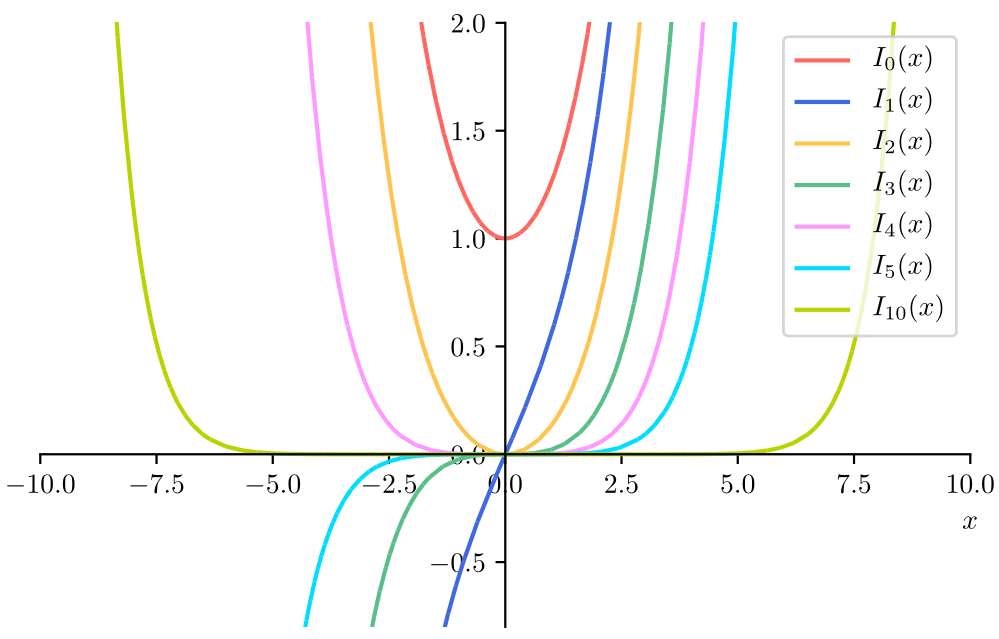
\includegraphics[width=75mm]{../fig/bessel/mod_bessel_n.png}
    \end{figure}
 \end{minipage}

 \begin{minipage}{0.50\hsize}
    \begin{figure}[H]
      \centering
      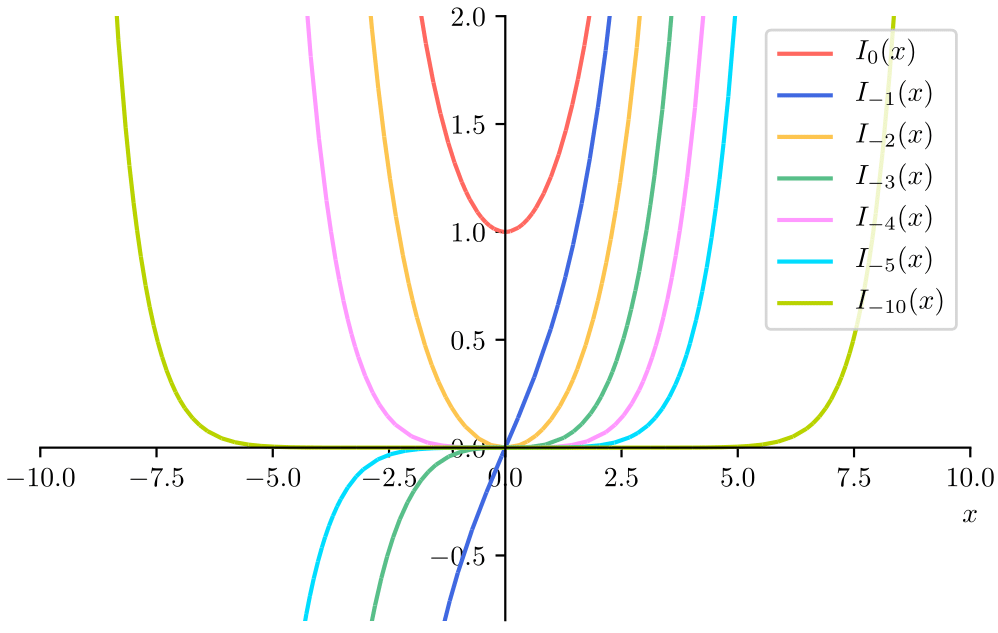
\includegraphics[width=75mm]{../fig/bessel/mod_bessel_n_minus.png}
    \end{figure}
 \end{minipage}
\end{tabular}

\begin{tabular}{cc}
\hspace{-22pt}
 \begin{minipage}{0.50\hsize}
    \begin{figure}[H]
      \centering
      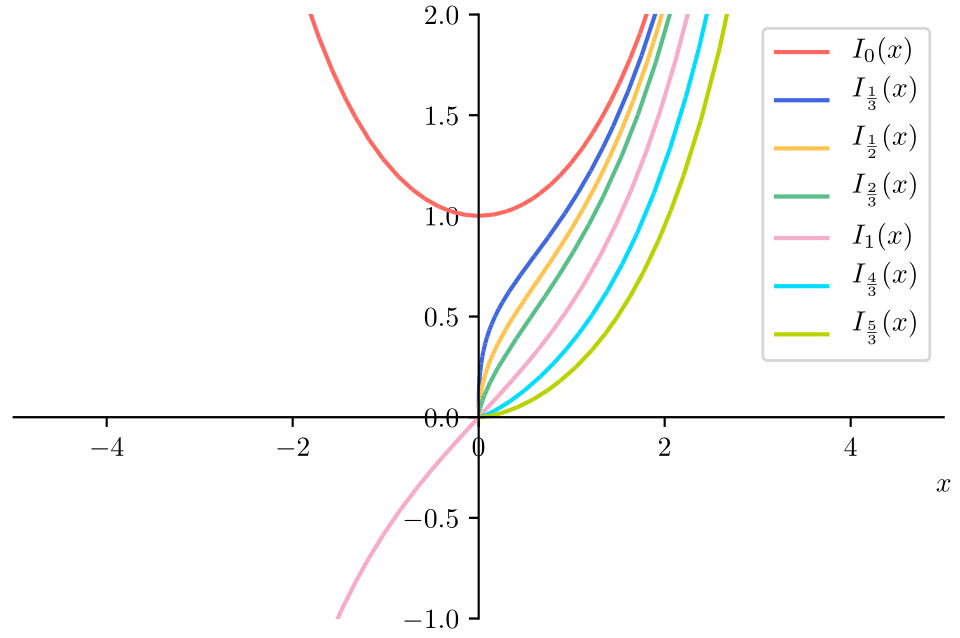
\includegraphics[width=75mm]{../fig/bessel/mod_bessel_nu.png}
    \end{figure}
 \end{minipage}

 \hspace{-4pt}
 \begin{minipage}{0.50\hsize}
    \begin{figure}[H]
      \centering
      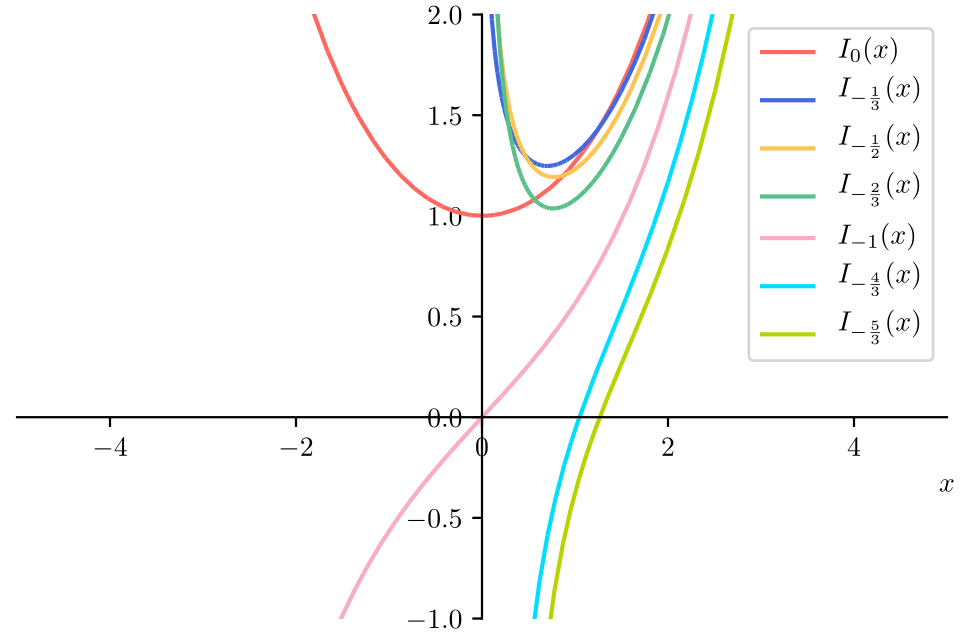
\includegraphics[width=75mm]{../fig/bessel/mod_bessel_nu_minus.png}
    \end{figure}
 \end{minipage}
\end{tabular}
\caption{第1種変形Bessel関数 $I_\nu(x)$}
\end{figure}

\subsubsection*{証明}

\paragraph{母関数}
Bessel関数の母関数
\begin{equation*}
  \tilde{g}(t, x) = e^{\frac{x}{2} \( t-\frac{1}{t} \)} 
	= \sum_{n=-\infty}^\infty J_n(x) t^n
\end{equation*}
において、$t \to -it, \ x\to ix$と置き換えて$g(t, x) \equiv \tilde{g}(-it, ix)$とすると
\begin{equation*}
  g(t, x) = e^{\frac{ix}{2} \( -it+\frac{1}{it} \)} 
	= \sum_{n=-\infty}^\infty J_n(ix) (-it)^n \qquad \therefore
  g(t, x) = e^{\frac{x}{2} \( t+\frac{1}{t} \)} 
	= \sum_{n=-\infty}^\infty i^{-n}J_n(ix) t^n 
\end{equation*}
変形Bessel関数の定義\eqref{eq:Inu-def}を用いて\eqref{eq:Inu-gene}を得る。\qed


\paragraph{偶奇性}
$J_{n} (-x) = (-1)^n J_n(x)$を用いて
\begin{align*}
  I_n(-x) = i^{-n} J_{n}(-ix)
	= i^{-n} (-1)^n J_n(ix)
	= (-1)^n I_n(x)
\end{align*}\qed

\paragraph{負の整数次}

$J_{-n}(x) = (-1)^n J_n(x)$を用いて
\begin{equation*}
  I_{-n}(x) = i^n J_{-n} (ix)
	= i^n (-1)^n J_{n} (ix)
	= i^n \cdot i^{-2n} J_n(ix)
	= i^{-n} J_n(ix)
	= I_n (x)
\end{equation*}\qed


\paragraph{一般項}
$J_\nu(x)$に関する一般項\eqref{eq:Jnu-ippan}を用いて
\begin{align*}
  I_\nu(x) &= i^{-\nu} J_\nu (ix) \notag\\
	&= i^{-\nu} \sum_{i=0}^\infty \frac{(-1)^i}{i!\ \Gamma(\nu +i+1)} \( \frac{ix}{2} \)^{\nu+2i} \notag\\
	&= \sum_{i=0}^\infty \frac{1}{i!\ \Gamma(\nu +i+1)} \( \frac{x}{2} \)^{\nu+2i}
\end{align*}\qed


\paragraph{漸化式}
$J_\nu(x)$に関する漸化式\eqref{eq:Jnu-req}において$x\to ix$とすると
\begin{equation*}
  \frac{2\nu}{ix} J_{\nu}(ix) = J_{\nu -1} (ix) + J_{\nu +1}(ix)
\end{equation*}
両辺を$i^{-\nu+1}$倍して
\begin{gather*}
  \frac{2\nu}{x} i^{-\nu} J_{\nu}(ix) 
		= i^{-(\nu-1)} J_{\nu -1} (ix) - i^{-(\nu+1)} J_{\nu +1}(ix) \qquad \therefore
  \frac{2\nu}{x} I_{\nu}(x) = I_{\nu -1} (x) - I_{\nu +1}(x)
\end{gather*}\qed


\paragraph{微分漸化式}
$J_\nu(x)$に関する微分漸化式\eqref{eq:Jnu-diff-req}において$x\to ix$とすると
\begin{equation*}
  2\frac{d J_\nu (ix)}{d(ix)} = J_{\nu -1}(ix) - J_{\nu +1} (ix)
\end{equation*}
両辺を$i^{-\nu+1}$倍して
\begin{gather*}
  2\frac{d \( i^{-\nu} J_\nu (ix) \) }{dx}
	=  i^{-(\nu-1)} J_{\nu -1} (ix) + i^{-(\nu+1)} J_{\nu +1}(ix) \qquad \therefore
  2\frac{d I_\nu (x)}{dx} = I_{\nu -1}(x) + I_{\nu +1} (x)
\end{gather*}\qed


\paragraph{下降演算子}
$J_\nu(x)$に関する下降演算子\eqref{eq:Jnu-kako}において$x\to ix$とすると
\begin{equation*}
  \( \frac{d}{d(ix)} + \frac{\nu}{ix} \) J_\nu (ix) = J_{\nu -1}(ix) 
\end{equation*}
両辺を$i^{-\nu+1}$倍して
\begin{gather*}
  \( \frac{d}{dx} + \frac{\nu}{x} \) i^{-\nu} J_\nu (ix) = i^{-(\nu-1)} J_{\nu -1}(ix)\qquad \therefore
  \( \dx{} + \frac{\nu}{x} \) I_\nu (x) = I_{\nu -1}(x)
\end{gather*}\qed


\paragraph{上昇演算子}
$J_\nu(x)$に関する上昇演算子\eqref{eq:Jnu-josho}において$x\to ix$とすると
\begin{equation*}
  \( \frac{d}{d(ix)} - \frac{\nu}{ix} \) J_\nu (ix) = - J_{\nu +1}(ix) 
\end{equation*}
両辺を$i^{-\nu+1}$倍して
\begin{gather*}
  \( \frac{d}{dx} - \frac{\nu}{x} \) i^{-\nu} J_\nu (ix) = i^{-(\nu+1)} J_{\nu +1}(ix)\qquad \therefore
  \( \dx{} - \frac{\nu}{x} \) I_\nu (x) = I_{\nu +1}(x)
\end{gather*}\qed


\paragraph{微分方程式}
$J_\nu(x)$に関する微分方程式\eqref{eq:Jnu-diff-eq}において$x\to ix$とすると
\begin{gather*}
  \frac{d^2 J_\nu (ix)}{d(ix)^2} + \frac{1}{ix} \frac{d J_\nu (ix)}{d(ix)} + \( 1-\frac{\nu^2}{(ix)^2} \) J_\nu (ix) = 0
  \notag\\ \therefore
  \frac{d^2 J_\nu (ix)}{dx^2} + \frac{1}{x} \frac{d J_\nu (ix)}{dx} - \( 1+\frac{\nu^2}{x^2} \) J_\nu (ix) = 0
\end{gather*}
両辺を$i^{-\nu}$倍して\eqref{eq:Inu-diff-eq1}を得る。

また、得られた微分方程式において$x\to kx$と置き換えると
\begin{gather*}
  \frac{d^2 I_\nu(kx)}{d(kx)^2} + \frac{1}{kx} \frac{d I_\nu(kx)}{d(kx)} - \( 1+\frac{\nu^2}{(kx)^2} \) I_\nu(kx) = 0
\end{gather*}
となり、
$\frac{d}{d(kx)} = \frac{1}{k} \dx{}$
に注意して整理すると\eqref{eq:Inu-diff-eq2}が得られる。
さらに\eqref{eq:Inu-diff-eq1}, \eqref{eq:Inu-diff-eq2}はそれぞれ\eqref{eq:Inu-self-1}, \eqref{eq:Inu-self-2}
のようにも書ける。
\qed


\paragraph{微分・積分公式}
$J_\nu(x)$に関する微分公式\eqref{eq:Jnu-bibun-1}において$x\to ix$とすると
\begin{equation*}
  \frac{d}{d(ix)} [(xi)^\nu J_\nu(ix)] = (ix)^\nu J_{\nu-1}(ix)
\end{equation*}
両辺を$i^{-2\nu+1}$倍して
\begin{equation*}
  \dx{} \[ x^\nu \cdot i^{-\nu} J_\nu(ix) \]
	= x^\nu \cdot i^{-\nu+1} J_{\nu-1} (ix) \qquad \therefore
  \dx{} [x^\nu I_\nu (x)] = x^\nu I_{\nu-1}(x)
\end{equation*}
これより積分公式は
\begin{equation*}
  \int x^\nu I_{\nu-1} (x) dx = x^\nu I_\nu (x) + C
\end{equation*}
\vspace{6pt}
同様に$J_\nu(x)$に関する微分公式\eqref{eq:Jnu-bibun-2}において$x\to ix$とすると
\begin{equation*}
  \frac{d}{d(ix)} [(ix)^{-\nu} J_\nu(ix)] = -(ix)^{-\nu} J_{\nu+1} (ix)
\end{equation*}
両辺を$i$倍して
\begin{equation*}
  \dx{} \[ x^{-\nu} \cdot i^{-\nu} J_\nu (ix) \]
	= x^{-\nu} \cdot i^{-\nu-1} J_{\nu+1} (ix) \qquad \therefore
  \dx{} \[ x^{-\nu} I_\nu(x) \] = x^{-\nu} I_{\nu+1} (x)
\end{equation*}
これより積分公式は
\begin{equation*}
  \int x^{-\nu} I_{\nu+1} (x) dx =  x^{-\nu} I_\nu(x) + C
\end{equation*}\qed

\paragraph{高階導関数表示}
$J_\nu(x)$に関する高階導関数表示\eqref{eq:Jnu-kokai-1}において$x\to ix$とすると
\begin{equation*}
(ix)^{-\nu-n} J_{\nu+n} (ix) = (-1)^n \( \frac{1}{ix} \frac{d}{d(ix)} \)^n \[ (ix)^{-\nu} J_\nu(ix) \] 
\end{equation*}
これより
\begin{equation*}
  x^{-\nu-n} \cdot i^{-\nu-n} J_{\nu+n} (ix)
	= \( \frac{1}{x} \dx{} \)^n \[ x^{-\nu} \cdot i^{-\nu} J_\nu (ix) \] \qquad \therefore
  x^{-\nu-n} I_{\nu+n} (x) = \( \frac{1}{x} \dx{} \)^n \[ x^{-\nu} I_\nu(x) \]
\end{equation*}
同様に$J_\nu(x)$に関する高階導関数表示\eqref{eq:Jnu-kokai-2}において$x\to ix$とすると
\begin{equation*}
  (ix)^{\nu-n} J_{\nu-n} (ix) = \( \frac{1}{ix} \frac{d}{d(ix)} \)^n \[ (ix)^\nu J_\nu(ix) \] 
\end{equation*}
両辺を$i^{-2\nu + 2n}$倍して
\begin{equation*}
  x^{\nu-n}\cdot i^{-\nu +n} J_{\nu-n}(ix)
	= \( \frac{1}{x} \dx{} \)^n \[ x^\nu \cdot i^{-\nu} J_\nu (ix) \] \qquad \therefore
  x^{\nu-n} I_{\nu-n} (x) = \( \frac{1}{x} \dx{} \)^n \[ x^\nu I_\nu(x) \]
\end{equation*}\qed



%%%%%%%%%%%%%%%%%%%%%%%%%%%%%%%%%%%%%%%%%%%%%%%%%%%%
\subsection{第2種変形Bessel関数}

変形されたBesselの微分方程式\eqref{eq:Inu-diff-eq1}についても
$I_\nu(x)$と線形独立なもうひとつの基本解を構成することを考える。
通常のBesselの微分方程式と同じ事情により、
$\nu$が整数でないときはもうひとつの基本解として$I_{-\nu}(x)$を選ぶことができるが、
$\nu$が整数であっても$I_\nu(x)$と線形独立になる基本解を得るためには
その代わりに\eqref{eq:Kn-def1}, \eqref{eq:Kn-def2}で定義される
第2種変形Bessel関数$K_\nu(x)$を用いることになる
\footnote{$I_\nu(x)とI_{-\nu}(x)$のロンスキアン $W[I_\nu, I_{-\nu}] (x)$、および
$I_\nu(x)とK_{\nu}(x)$のロンスキアン $W[I_\nu, K_{\nu}] (x)$はそれぞれ
\begin{align}
  &W[I_\nu, I_{-\nu}] (x) = I_\nu (x) I_{-\nu}^\prime(x) - I_\nu^\prime(x) I_{-\nu}(x)
	= -\frac{2\sin \pi\nu}{\pi x} \\
  &W[I_\nu, K_{\nu}] (x) = I_\nu (x) K_{\nu}^\prime (x) - I_\nu^\prime(x) K_{\nu}(x)
	= -\frac{1}{x} 
\end{align}
}
。
$K_\nu(x)$についての微分方程式は$I_\nu(x)$の場合と一致するが、
\textbf{漸化式、微分漸化式、昇降演算子は符号が逆になっている}ことに注意を要する。
各公式の証明は$N_\nu(x)$のときの方法とほとんど同じである。
なお$K_\nu(x)$は\eqref{eq:Kn-H}のようにHankel関数で表すこともできる。

\subsubsection*{公式集}

\paragraph{定義}
\begin{alignat}{2}
  &K_\nu (x) = \frac{\pi}{2} \frac{I_{-\nu} (x) - I_{\nu}(x) }{ \sin\pi\nu} &\qquad & (\nu \notin \mathbb{Z})
	\label{eq:Kn-def1}\\
  &K_n (x) = \lim_{\nu\to n} I_\nu (x) & & (\nu = n \in \mathbb{Z})
	\label{eq:Kn-def2}
\end{alignat}

\paragraph{Hankel関数表示}
\begin{equation}\label{eq:Kn-H}
  K_\nu (x) = \frac{\pi}{2} i^{\nu+1} H_\nu^{(1)} (ix)
\end{equation}


\paragraph{整数次の表式}
\begin{equation}\label{eq:Knu-hyo}
  K_n (x) = \frac{(-1)^n}{2} \[ \frac{\6 I_{-\nu} (x)}{\6 \nu} - \frac{\6 I_{\nu} (x)}{\6 \nu} \]_{\nu =n}
\end{equation}

\paragraph{非負整数次の一般項(参考)}
\begin{align}
  K_n(x) &= (-1)^{n+1} I_n(x) \log \frac{x}{2} \notag\\
	&\hspace{24pt} + \frac{(-1)^n}{2} \sum_{i=0}^\infty \frac{1}{i! (n+i)!} \( \frac{x}{2} \)^{n+2i}
		\[ \psi (i+1) + \psi(n+i+1) \] \notag\\
	&\hspace{24pt} + \frac{1}{2} \sum_{i=0}^{n-1} (-1)^i \frac{(n-i-1)!}{i!} \( \frac{x}{2} \)^{-n+2i}
		\qquad (n= 0, 1, 2, \dots)
\end{align}

\paragraph{負の次数}
\hspace{-6pt}\footnote{$N_\nu(x)$のときとは異なり、これは$\nu$が整数でない一般の場合でも成立する。}
\begin{equation}
  K_{-\nu} (x) = K_\nu (x)
\end{equation}

\paragraph{漸化式}
\begin{equation}\label{eq:Knu-req}
  -\frac{2\nu}{x} K_{\nu}(x) = K_{\nu -1} (x) - K_{\nu +1}(x)
\end{equation}

\paragraph{微分漸化式}
\begin{equation}\label{eq:Knu-req-diff}
  -2\frac{d K_\nu (x)}{dx} = K_{\nu -1}(x) + K_{\nu +1} (x)
\end{equation}

\paragraph{昇降演算子}
\begin{alignat}{2}
  &\mathrm{\textbf{下降演算子}} & \quad & \( \dx{} + \frac{\nu}{x} \) K_\nu (x) = -K_{\nu -1}(x) 
		\label{eq:Knu-kako}\\
  &\mathrm{\textbf{上昇演算子}} &  & \( \dx{} - \frac{\nu}{x} \) K_\nu (x) =  -K_{\nu +1}(x) 
		\label{eq:Knu-josho}
\end{alignat}

\paragraph{微分方程式}
\begin{gather}
  \frac{d^2 K_\nu (x)}{dx^2} + \frac{1}{x} \frac{d K_\nu (x)}{dx} - \( 1+\frac{\nu^2}{x^2} \) K_\nu (x) = 0
	\label{eq:Knu-diff-eq1}\\
  \frac{d^2 K_\nu (kx)}{dx^2} + \frac{1}{x} \frac{d K_\nu (kx)}{dx} - \( k^2+\frac{\nu^2}{x^2} \) K_\nu (kx) = 0
	\label{eq:Knu-diff-eq2}
\end{gather}

\paragraph{自己随伴形}
\begin{gather}
  \dx{} \[ x \dx{} K_\nu (x) \] - \( x + \frac{\nu^2}{x} \) K_\nu (x) = 0 \label{eq:Knu-self-1}\\
  \dx{} \[ x \dx{} K_\nu (kx) \] - \( k^2 x + \frac{\nu^2}{x} \) K_\nu (kx) = 0 \label{eq:Knu-self-2} 
\end{gather}

\paragraph{微分・積分公式}
\begin{alignat}{2}
  \dx{} [x^\nu K_\nu(x)] &= - x^\nu K_{\nu-1}(x) , 
		&  \int x^\nu K_{\nu-1}(x) dx &= -x^\nu K_\nu(x) + C \label{eq:Knu-bibun-1}\\
  \dx{} [x^{-\nu} K_\nu(x)] &= -x^{-\nu} K_{\nu+1} (x) , 
		&\quad\qquad \int x^{-\nu} K_{\nu+1} (x) dx &=  -x^{-\nu} K_\nu(x) + C
  \label{eq:Knu-bibun-2}
\end{alignat}

\paragraph{高階導関数表示}
$n=0, 1, 2, \dots$とすると
\begin{align}
  x^{-\nu-n} K_{\nu+n} (x) &= (-1)^n \( \frac{1}{x} \dx{} \)^n \[ x^{-\nu} K_\nu(x) \]
	\label{eq:Knu-kokai-1} \\
  x^{\nu-n} K_{\nu-n} (x) &= (-1)^n \( \frac{1}{x} \dx{} \)^n \[ x^\nu K_\nu(x) \]
	\label{eq:Knu-kokai-2}
\end{align}


% 図
\begin{figure}[tb]
\begin{tabular}{cc}
\hspace{-24pt}
 \begin{minipage}{0.50\hsize}\small
    \begin{figure}[H]
      \centering
      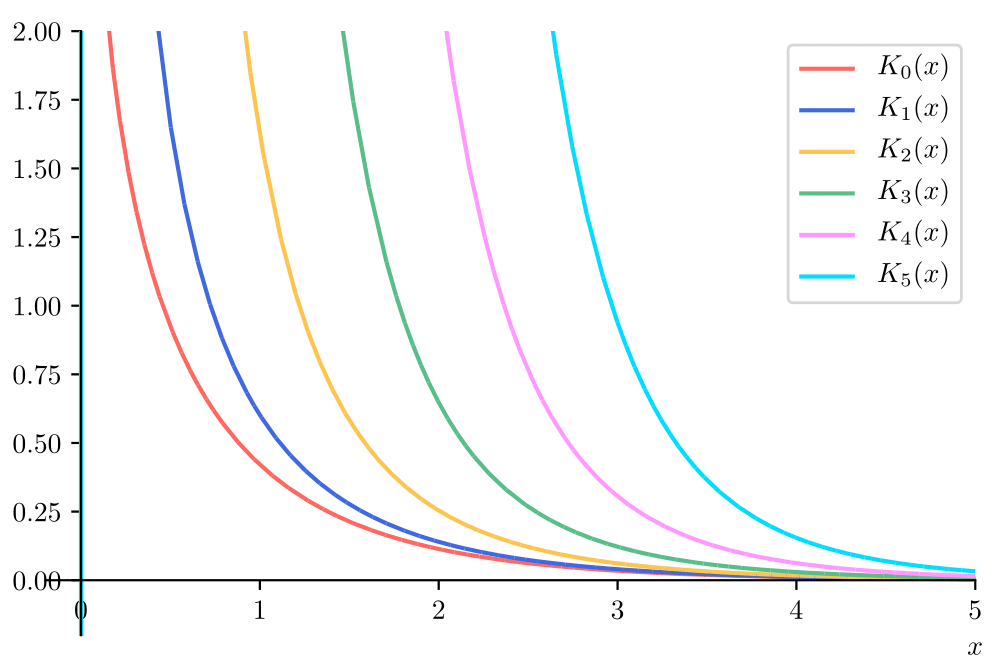
\includegraphics[width=75mm]{../fig/bessel/mod_K_n.png}
    \end{figure}
 \end{minipage}

 \begin{minipage}{0.50\hsize}
    \begin{figure}[H]
      \centering
      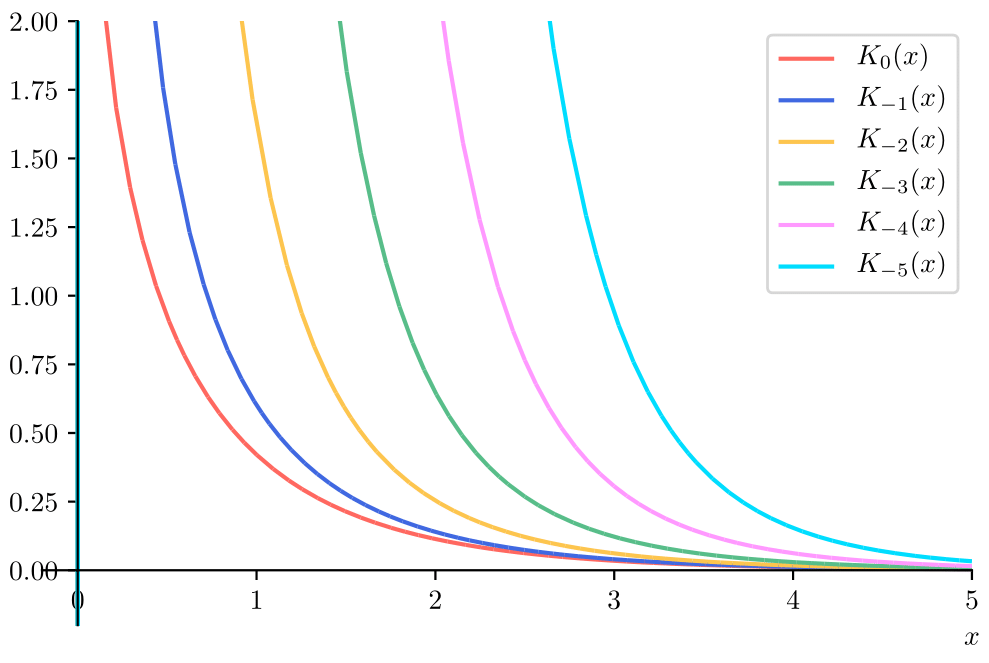
\includegraphics[width=75mm]{../fig/bessel/mod_K_n_minus.png}
    \end{figure}
 \end{minipage}
\end{tabular}

\begin{tabular}{cc}
\hspace{-25pt}
 \begin{minipage}{0.50\hsize}
    \begin{figure}[H]
      \centering
      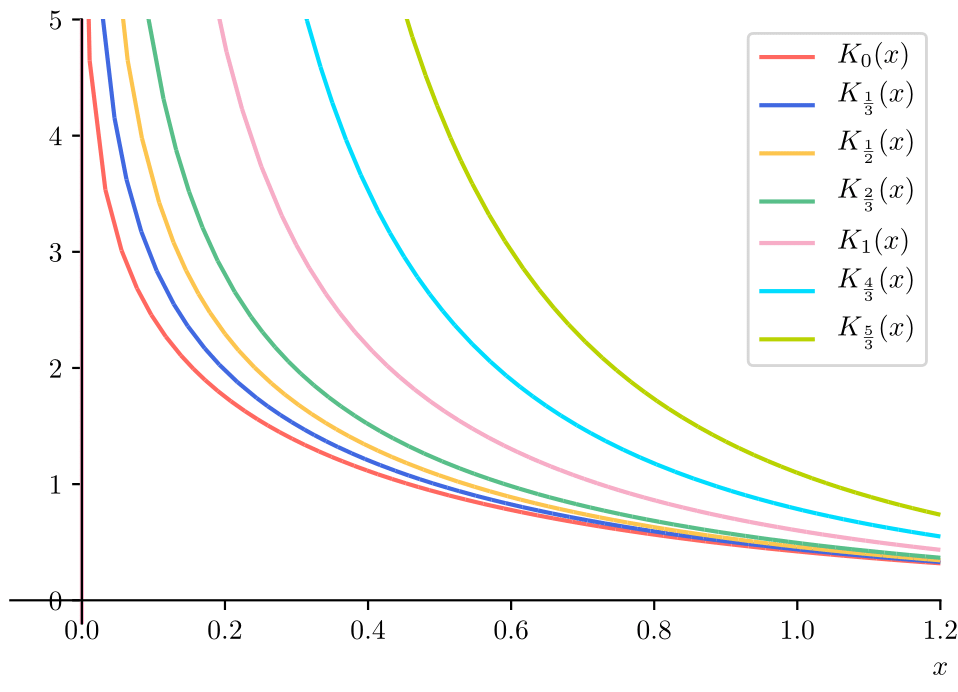
\includegraphics[width=75mm]{../fig/bessel/mod_K_nu.png}
    \end{figure}
 \end{minipage}

 \hspace{-4pt}
 \begin{minipage}{0.50\hsize}
    \begin{figure}[H]
      \centering
      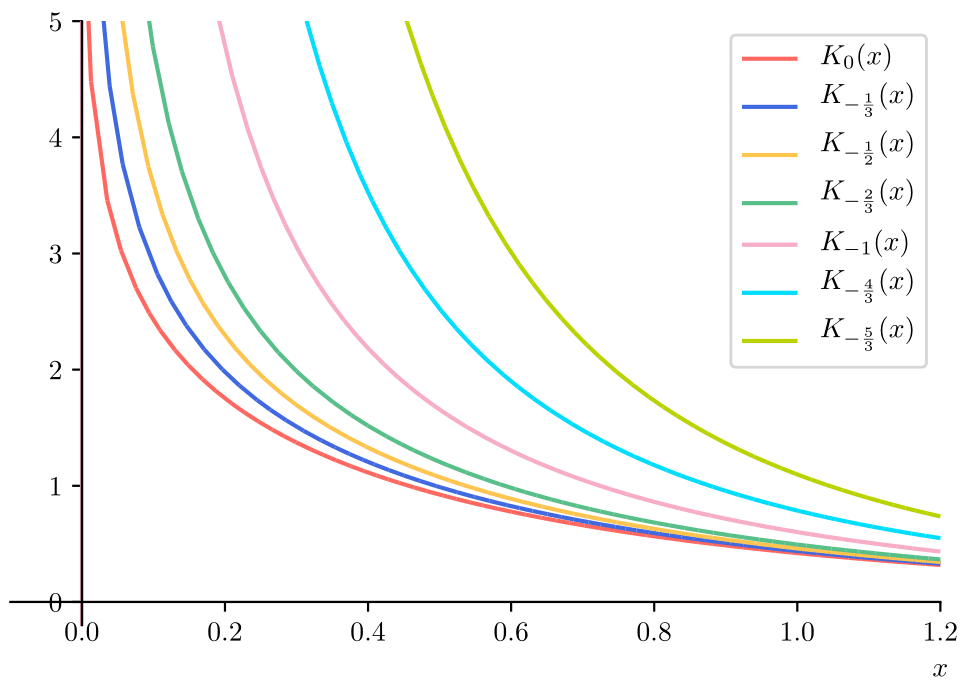
\includegraphics[width=75mm]{../fig/bessel/mod_K_nu_minus.png}
    \end{figure}
 \end{minipage}
\end{tabular}
\caption{第2種変形Bessel関数 $K_\nu(x)$}
\end{figure}



\subsubsection*{証明}

\paragraph{定義 $\Longrightarrow$ Hankel関数表示}
$I_\nu(x)$の定義\eqref{eq:Inu-def}を用いて$K_\nu(x)$を$J_\nu(x)$で表すと
\begin{align*}
  K_\nu(x) &= \frac{\pi}{2} \frac{I_{-\nu} (x) - I_{\nu}(x) }{ \sin\pi\nu} 
	 = \frac{\pi}{2} \frac{i^\nu J_{-\nu} (ix) - i^{-\nu} J_{\nu}(ix) }{ \sin\pi\nu} \notag\\
	&= \frac{\pi}{2} i^{\nu+1} \cdot \frac{ i^{-2\nu+1} J_{\nu}(ix)  - i J_{-\nu}(ix) }{\sin\pi\nu}
\end{align*}
ここで
\begin{equation*}
  i^{-2\nu+1}
	= i \cdot i^{-2\nu}
	= i e^{-i\pi\nu}
	= i (\cos\pi\nu - i \sin\pi\nu )
	= \sin\pi\nu + i\cos\pi\nu
\end{equation*}
であるから、
\begin{align*}
  K_\nu(x)
	&= \frac{\pi}{2} i^{\nu+1} \cdot \[ J_\nu (ix) 
		+ i \cdot \frac{J_\nu(ix)\cos\pi\nu - J_{-\nu} (ix)}{\sin\pi\nu} \] \notag\\
	&= \frac{\pi}{2} i^{\nu+1} \( J_\nu(ix) + i N_\nu(ix) \) 
	= \frac{\pi}{2} i^{\nu+1} H_\nu^{(1)} (ix)
\end{align*}\qed


\paragraph{定義 $\Longrightarrow$ 整数次の表式}
極限\eqref{eq:Kn-def2}は$\frac{0}{0}$不定形であるのでL'H\^opitalの定理を用いることができる。
\begin{align*}
  K_n(x) &= \lim_{\nu\to n} \frac{\pi}{2} \frac{I_{-\nu} (x) - I_{\nu}(x) }{ \sin\pi\nu} 
	= \lim_{\nu\to n} \frac{\pi}{2} \frac{\frac{\6 I_{-\nu} (x)}{\6\nu} 
		- \frac{\6 I_{\nu}(x)}{\6\nu} }{ \pi\cos\pi\nu} \notag\\
	&= \frac{(-1)^n}{2} \[ \frac{\6 I_{-\nu} (x)}{\6 \nu} - \frac{\6 I_{\nu} (x)}{\6 \nu} \]_{\nu =n}
\end{align*}\qed



\paragraph{定義 $\Longrightarrow$ 負の次数}
定義\eqref{eq:Kn-def1}において$\nu$を$-\nu$に置き換えても式は変わらないので
\begin{equation*}
  K_{-\nu} (x) = K_\nu (x)
\end{equation*}\qed


\paragraph{定義 $\Longrightarrow$ 漸化式}
$\nu\notin\mathbb{Z}$のとき、\eqref{eq:Kn-def1}から
\begin{align*}
  &\hspace{-24pt} K_{\nu -1} (x) - K_{\nu +1}(x)\notag\\
	&= \frac{\pi}{2} \frac{I_{-\nu+1} (x) - I_{\nu-1}(x) }{ \sin\pi(\nu-1)}
		- \frac{\pi}{2} \frac{I_{-\nu-1} (x) - I_{\nu+1}(x) }{ \sin\pi(\nu+1)} \notag\\
	&= \frac{\pi}{2} \frac{- I_{-\nu+1} (x) + I_{\nu-1}(x) }{ \sin\pi\nu}
		- \frac{\pi}{2} \frac{-I_{-\nu-1} (x) + I_{\nu+1}(x) }{ \sin\pi\nu} \notag\\
	&= \frac{\pi}{2} \frac{\( I_{-\nu-1} (x) - I_{-\nu+1} (x) \) 
				+ \( I_{\nu-1} (x) - I_{\nu+1} (x) \) }{\sin\pi\nu} \notag\\
	&= -\frac{2\nu}{x} \cdot \frac{\pi}{2} \frac{I_{-\nu} (x) - I_{\nu}(x) }{ \sin\pi\nu} \notag\\
	&= -\frac{2\nu}{x} K_\nu(x)
\end{align*}
次に$\nu =n\in\mathbb{Z}$のとき、\eqref{eq:Knu-hyo}から
\begin{align*}
  &\hspace{-24pt} K_{n -1} (x) - K_{n +1}(x) \notag\\
	&= \frac{(-1)^{n-1}}{2} \[ \frac{\6 I_{-\nu} (x)}{\6 \nu} - \frac{\6 I_{\nu} (x)}{\6 \nu} \]_{\nu =n-1}
	- \frac{(-1)^{n+1}}{2} \[ \frac{\6 I_{-\nu} (x)}{\6 \nu} - \frac{\6 I_{\nu} (x)}{\6 \nu} \]_{\nu =n+1}\notag\\
	&= \frac{(-1)^n}{2} \[ - \frac{\6 I_{-\nu+1} (x)}{\6 \nu} + \frac{\6 I_{\nu-1} (x)}{\6 \nu}
		+ \frac{\6 I_{-\nu-1} (x)}{\6 \nu} - \frac{\6 I_{\nu+1} (x)}{\6 \nu} \]_{\nu=n} \notag\\
	&= \frac{(-1)^n}{2} \[ \frac{\6}{\6 \nu} \( I_{-\nu-1}(x) - I_{-\nu+1}(x) \) 
		+ \frac{\6}{\6 \nu} \( I_{\nu-1}(x) - I_{\nu+1} (x) \) \]_{\nu=n} \notag\\
	&= \frac{(-1)^n}{2} \[ \frac{\6}{\6 \nu} \( \frac{-2\nu}{x} I_{-\nu}(x) \)
		+ \frac{\6}{\6 \nu} \( \frac{2\nu}{x} I_\nu (x) \) \]_{\nu=n} \notag\\
	&= \frac{(-1)^n}{2} \[ -\frac{2}{x} I_{-\nu}(x) - \frac{2\nu}{x} \frac{\6 I_{-\nu}(x)}{\6 \nu} 
		+ \frac{2}{x} I_\nu(x) + \frac{2\nu}{x} \frac{\6 I_\nu(x)}{\6 \nu} \]_{\nu=n} \notag\\
	&= -\frac{2n}{x} \cdot \frac{(-1)^n}{2} \[ \frac{\6 I_{-\nu} (x)}{\6 \nu} 
		- \frac{\6 I_{\nu} (x)}{\6 \nu}  \]_{\nu=n}\notag\\
	&= -\frac{2n}{x} K_n(x)
\end{align*}\qed


\paragraph{定義 $\Longrightarrow$ 微分漸化式}
$\nu\notin\mathbb{Z}$のとき、\eqref{eq:Kn-def1}から
\begin{align*}
  &\hspace{-24pt} K_{\nu -1} (x) + K_{\nu +1}(x)\notag\\
	&= \frac{\pi}{2} \frac{I_{-\nu+1} (x) - I_{\nu-1}(x) }{ \sin\pi(\nu-1)}
		+ \frac{\pi}{2} \frac{I_{-\nu-1} (x) - I_{\nu+1}(x) }{ \sin\pi(\nu+1)} \notag\\
	&= \frac{\pi}{2} \frac{- I_{-\nu+1} (x) + I_{\nu-1}(x) }{ \sin\pi\nu}
		+ \frac{\pi}{2} \frac{-I_{-\nu-1} (x) + I_{\nu+1}(x) }{ \sin\pi\nu} \notag\\
	&= -\frac{\pi}{2} \frac{\( I_{-\nu-1} (x) + I_{-\nu+1} (x) \) 
				- \( I_{\nu-1} (x) + I_{\nu+1} (x) \) }{\sin\pi\nu} \notag\\
	&= -2\dx{} \cdot \frac{\pi}{2} \frac{I_{-\nu} (x) - I_{\nu}(x) }{ \sin\pi\nu} \notag\\
	&= -2 \frac{d K_\nu(x)}{dx}
\end{align*}
次に$\nu =n\in\mathbb{Z}$のとき、\eqref{eq:Knu-hyo}から
\begin{align*}
  &\hspace{-24pt} K_{n -1} (x) + K_{n +1}(x) \notag\\
	&= \frac{(-1)^{n-1}}{2} \[ \frac{\6 I_{-\nu} (x)}{\6 \nu} - \frac{\6 I_{\nu} (x)}{\6 \nu} \]_{\nu =n-1}
	+ \frac{(-1)^{n+1}}{2} \[ \frac{\6 I_{-\nu} (x)}{\6 \nu} - \frac{\6 I_{\nu} (x)}{\6 \nu} \]_{\nu =n+1}\notag\\
	&= -\frac{(-1)^n}{2} \[ \frac{\6 I_{-\nu+1} (x)}{\6 \nu} - \frac{\6 I_{\nu-1} (x)}{\6 \nu}
		+ \frac{\6 I_{-\nu-1} (x)}{\6 \nu} - \frac{\6 I_{\nu+1} (x)}{\6 \nu} \]_{\nu=n} \notag\\
	&= -\frac{(-1)^n}{2} \[ \frac{\6}{\6 \nu} \( I_{-\nu-1}(x) + I_{-\nu+1}(x) \) 
		- \frac{\6}{\6 \nu} \( I_{\nu-1}(x) + I_{\nu+1} (x) \) \]_{\nu=n} \notag\\
	&= -\frac{(-1)^n}{2} \[ \frac{\6}{\6 \nu} \( 2\frac{d I_{-\nu}(x)}{dx} \)
		- \frac{\6}{\6 \nu} \( 2\frac{d I_\nu (x)}{dx} \) \]_{\nu=n} \notag\\
	&= -2\dx{} \frac{(-1)^n}{2} \[ \frac{\6 I_{-\nu} (x)}{\6 \nu} 
		- \frac{\6 I_{\nu} (x)}{\6 \nu}  \]_{\nu=n}\notag\\
	&= -2\frac{d K_n(x)}{dx}
\end{align*}\qed


\paragraph{漸化式, 微分漸化式 $\Longrightarrow$ 昇降演算子}
まず下降演算子については$-\frac{1}{2}\[ \eqref{eq:Knu-req-diff}+\eqref{eq:Knu-req} \]$を計算して
\begin{equation*}
  \( \dx{} + \frac{\nu}{x} \) K_\nu (x) = -K_{\nu -1}(x)
\end{equation*}
上昇演算子については$-\frac{1}{2} \[ \eqref{eq:Knu-req-diff}-\eqref{eq:Knu-req} \] $を計算して
\begin{equation*}
  \( \dx{} - \frac{\nu}{x} \) K_\nu (x) =  -K_{\nu +1}(x) 
\end{equation*}\qed


\paragraph{昇降演算子 $\Longrightarrow$ 微分方程式}
上昇演算子\eqref{eq:Knu-josho}の両辺に左から$\dx{} + \frac{\nu+1}{x}$を作用させると、左辺は
\begin{align*}
  \( \dx{} + \frac{\nu+1}{x} \) \( \dx{} - \frac{\nu}{x} \) K_\nu (x)
	&= \[ \dx{} \( \dx{} - \frac{\nu}{x} \) + \frac{\nu+1}{x} \( \dx{} - \frac{\nu}{x} \) \] K_\nu (x)\notag\\
	&= \[ \( \dx{2} + \frac{\nu}{x^2}-\frac{\nu}{x}\dx{} \) 
		+ \( \frac{\nu+1}{x} \dx{} - \frac{\nu^2+\nu}{x^2} \) \] K_\nu (x)\notag\\
	&= \( \dx{2} + \frac{1}{x} \dx{} - \frac{\nu^2}{x^2} \) K_\nu(x)
\end{align*}
一方右辺は$- \( \dx{} + \frac{\nu+1}{x} \) K_{\nu+1}(x)$であるがこれは
下降演算子\eqref{eq:Knu-kako}から$K_\nu(x)$に等しい。よって、
\begin{equation*}
  \( \dx{2} + \frac{1}{x} \dx{} - \frac{\nu^2}{x^2} \) K_\nu(x) = K_\nu(x) \qquad\therefore
	\frac{d^2 K_\nu (x)}{dx^2} + \frac{1}{x} \frac{d K_\nu (x)}{dx} - \( 1+\frac{\nu^2}{x^2} \) K_\nu (x) = 0
\end{equation*}
また、得られた微分方程式において$x\to kx$と置き換えると
\begin{gather*}
  \frac{d^2 K_\nu(kx)}{d(kx)^2} + \frac{1}{kx} \frac{d K_\nu(kx)}{d(kx)} - \( 1+\frac{\nu^2}{(kx)^2} \) K_\nu(kx) 
	= 0
\end{gather*}
となり、
$\frac{d}{d(kx)} = \frac{1}{k} \dx{}$
に注意して整理すると\eqref{eq:Knu-diff-eq2}が得られる。
さらに\eqref{eq:Knu-diff-eq1}, \eqref{eq:Knu-diff-eq2}はそれぞれ\eqref{eq:Knu-self-1}, \eqref{eq:Knu-self-2}
のようにも書ける。
\qed


\paragraph{昇降演算子 $\Longrightarrow$ 微分・積分公式}

下降演算子\eqref{eq:Knu-kako}の両辺に$x^\nu$をかけると

\begin{equation*}
  \( x^\nu \dx{} + \nu x^{\nu-1} \) K_\nu(x) = - x^\nu K_{\nu-1}(x) \qquad \therefore
	\dx{} [x^\nu K_\nu(x)] = - x^\nu K_{\nu-1} (x)
\end{equation*}
これより積分公式は
\begin{equation*}
  \int x^\nu K_{\nu-1} (x) dx = - x^\nu K_\nu (x) + C
\end{equation*}
同様に上昇演算子\eqref{eq:Knu-josho}の両辺に$x^{-\nu}$をかけると
\begin{equation*}
  \( x^{-\nu} \dx{} - \nu x^{-\nu-1} \) K_\nu(x) =  - x^{-\nu} K_{\nu+1}(x) \qquad \therefore
	\dx{} [x^{-\nu} K_\nu(x)] = -x^{-\nu} K_{\nu+1} (x) 
\end{equation*}
これより積分公式は
\begin{equation*}
  \qquad \int x^{-\nu} K_{\nu+1} (x) dx = - x^{-\nu} K_\nu(x) + C
\end{equation*}\qed

\paragraph{微分公式 $\Longrightarrow$ 高階導関数表示}
\eqref{eq:Knu-bibun-2}の微分公式の両辺を$x$でわって
\begin{equation*}
  \frac{1}{x} \dx{} [x^{-\nu} K_\nu(x)] = -x^{-\nu-1} K_{\nu+1} (x)
\end{equation*}
と変形すると、関数$x^{-\nu} K_\nu(x)$に1回$\frac{1}{x} \dx{}$を作用させると
$x$の指数が1減り、第2種変形Bessel関数の次数が1増え、符号が反転することが読み取れる。
したがって$x^{-\nu} K_\nu(x)$に対して$\frac{1}{x} \dx{}$を$n$回作用させると
\begin{equation*}
  \( \frac{1}{x} \dx{} \)^n [x^{-\nu} K_\nu(x)] = (-1)^n x^{-\nu-n} K_{\nu+n} (x)
\end{equation*}
となることが分かり、\eqref{eq:Knu-kokai-1}が示される。
同様に\eqref{eq:Knu-bibun-1}の微分公式の両辺を$x$でわって
\begin{equation*}
  \frac{1}{x} \dx{} [x^\nu K_\nu(x)] = - x^{\nu-1} K_{\nu-1}(x)
\end{equation*}
と変形すると、関数$x^\nu K_\nu(x)$に1回$\frac{1}{x} \dx{}$を作用させると
$x$の指数と第2種変形Bessel関数の次数がともに1ずつ減り、符号が反転することが読み取れるので、
$x^\nu K_\nu(x)$に対して$\frac{1}{x} \dx{}$を$n$回作用させると
\begin{equation*}
  \( \frac{1}{x} \dx{} \)^n [x^\nu K_\nu(x)] = (-1)^n x^{\nu-n} K_{\nu-n}(x)
\end{equation*}
となることが分かり、\eqref{eq:Knu-kokai-2}が示される。\qed






\subsection{変形Bessel関数まとめ}

変形されたBesselの微分方程式
\begin{equation}
  \frac{d^2 y}{dx^2} + \frac{1}{x} \frac{dy}{dx} - \( 1+\frac{\nu^2}{x^2} \)y = 0
\end{equation}
の一般解は、
\vspace{6pt}
\begin{enumerate}
  \item $\nu$が整数でないならば
  \begin{equation}
    y = c_1 I_\nu (x) + c_2 I_{-\nu} (x)
  \end{equation}
  \item 一般には
  \begin{equation}
    y = c_1 I_\nu (x) + c_2 K_\nu (x)
  \end{equation}
\end{enumerate}
と書ける。

\subsection{漸近形(参考)}

\paragraph{漸近形}
十分大きな$x$に対して
\begin{align}
  I_\nu (x) &\sim \frac{e^x}{\sqrt{2\pi x}} \\
  K_\nu(x) &\sim \sqrt{\frac{\pi}{2x}} e^{-x}
\end{align}


%%%%%%%%%%%%%%%%%%%%%%%%%%%%%%%%%%%%%%%%%%%%%%%%%%%%%%%%%%%%%%%%%
\section{球Bessel関数}
\subsection{球Bessel関数}
球Bessel関数(第1種球Bessel関数) $j_n(x)$,  球Neumann関数(第2種球Bessel関数) $n_n(x)$, 
第1種球Hankel関数$h_n^{(1)}(x)$, 第2種球Hankel関数$h_n^{(2)}(x)$を総称して
球Bessel関数と呼び、$z_n(x)$と書くことにする。
$z_n(x)$は対応する円柱関数$Z_\nu(x)$を用いて$z_n(x) = \sqrt{\frac{\pi}{2x}} Z_{n+\frac{1}{2}}(x)$と定義され、
多くの物理系では$n=0, 1, 2, \dots$の場合が問題とされる。

球Bessel関数では高階導関数表示が重要であり、
これによれば$z_n(x)$が初等関数である三角関数や指数関数で書けることが読み取れる。
これは円柱関数$Z_\nu(x)$が一般に初等関数で書けないことと対照的である。
高階導関数表示は球Bessel関数$z_n(x)$がどのような初等関数で書けるか理解しやすいため、
これを定義として採用する教科書も多い。

球Bessel関数は円柱関数の特殊な場合であるので、
$z_n(x)$についての諸公式は一般次数の円柱関数$Z_\nu(x)$の諸公式から演繹できる。
特に高階導関数表示、漸化式、微分漸化式、昇降演算子、微分方程式が任意の球Bessel関数$z_n(x)$について
共通であることは注目に値する。


\subsection*{公式集}

\paragraph{定義} \hspace{-10pt}
\footnote{
\eqref{eq:nn-def}で
$\sqrt{\frac{\pi}{2x}} N_{n+\frac{1}{2}} (x) 
		= (-1)^{n+1} \sqrt{\frac{\pi}{2x}} J_{-n-\frac{1}{2}} (x)$
であることはNeumann関数$N_\nu(x)$の定義\eqref{eq:Nnu-def1}を用いて確かめられる。
}
\begin{subnumcases}
{z_n(x) = \sqrt{\frac{\pi}{2x}} Z_{n+\frac{1}{2}} (x)   \quad }
  j_n(x) = \sqrt{\frac{\pi}{2x}} J_{n+\frac{1}{2}} (x) & \\
  n_n (x) = \sqrt{\frac{\pi}{2x}} N_{n+\frac{1}{2}} (x) 
		= (-1)^{n+1} \sqrt{\frac{\pi}{2x}} J_{-n-\frac{1}{2}} (x) & \label{eq:nn-def}\\
  h_n^{(1)} (x) = \sqrt{\frac{\pi}{2x}} H_{n+\frac{1}{2}}^{(1)} (x)
		= j_n(x) + i \, n_n(x) & \\
  h_n^{(2)} (x) = \sqrt{\frac{\pi}{2x}} H_{n+\frac{1}{2}}^{(2)} (x) 
		= j_n(x) - i \, n_n(x) &
\end{subnumcases}

\paragraph{一般項}
\begin{align}
  j_n(x) &= 2^n x^n \sum_{i=0}^\infty \frac{(-1)^i (n+i)!}{i! \, (2n+2i+1)!} x^{2i} \label{eq:jn-ippan}\\
  n_n(x) &= -\frac{1}{2^n x^{n+1}} \[ 
	\sum_{i=0}^{n} \frac{(2n-2i)!}{i! \, (n-i)!} x^{2i}
		+ (-1)^n \sum_{i=n+1}^\infty \frac{(-1)^i (-n+i)!}{i!\, (-2n+2i)!} x^{2i}
	 \] \label{eq:nn-ippan} \\
		&= -\frac{1}{2^n x^{n+1}} \[ 
	\sum_{i=0}^{n-1} \frac{(2n-2i)!}{i! \, (n-i)!} x^{2i}
		+ (-1)^n \sum_{i=n}^\infty \frac{(-1)^i (-n+i)!}{i!\, (-2n+2i)!} x^{2i}
	 \] \label{eq:nn-ippan-2} 
\end{align}

\paragraph{$x\sim 0$での振舞}
\begin{align}
  j_n (x) &\sim \frac{x^n}{(2n+1)!!} \\
  n_n(x) &\sim - \frac{(2n-1)!!}{x^{n+1}}
\end{align}

\paragraph{$n=0$の表式}
\begin{align}
  j_0(x) &= \frac{\sin x}{x} \\
  n_0(x) &= -\frac{\cos x}{x} \\
  h_0^{(1)}(x) &= -i \frac{e^{ix}}{x} \\
  h_0^{(2)}(x) &= i\frac{e^{-ix}}{x}
\end{align}


\paragraph{高階導関数表示}
\begin{alignat}{2}
  j_n(x) &= (-1)^n x^n \( \frac{1}{x} \dx{} \)^n j_0(x), & \qquad & j_0(x) = \frac{\sin x}{x} \\
  n_n(x) &=  (-1)^n x^n \( \frac{1}{x} \dx{} \)^n n_0(x), & \qquad & n_0(x) = - \frac{\cos x}{x} \\
  h_n^{(1)}(x) &=  (-1)^n x^n \( \frac{1}{x} \dx{} \)^n h_0^{(1)} (x), 
		& \qquad & h_0^{(1)}(x) = - i \frac{e^{ix}}{x}\\
  h_n^{(2)}(x) &=  (-1)^n x^n \( \frac{1}{x} \dx{} \)^n h_0^{(2)} (x), 
		& \qquad & h_0^{(2)}(x) =  i \frac{e^{-ix}}{x}
\end{alignat}

\paragraph{漸化式}
\begin{equation}\label{eq:zn-req}
  \frac{2n+1}{x} z_n(x) = z_{n-1} (x) + z_{n-1} (x) 
\end{equation}

\paragraph{微分漸化式}
\begin{equation}\label{eq:zn-req-diff}
  \( 2\dx{} + \frac{1}{x} \) z_n(x) = z_{n-1}(x) - z_{n+1} (x)
\end{equation}

\paragraph{昇降演算子}
\begin{alignat}{2}
  &\textbf{下降演算子} &\qquad & \( \dx{} + \frac{n+1}{x} \) z_n(x) = z_{n-1} (x) \label{eq:zn-kako}\\ 
  &\textbf{上昇演算子} &\qquad & \( \dx{} - \frac{n}{x} \) z_n(x) = -z_{n+1} (x) \label{eq:zn-josho}
\end{alignat}


\paragraph{微分方程式}
\begin{gather}
  \frac{d^2 z_n(x)}{dx^2} + \frac{2}{x} \frac{d z_n(x)}{dx} 
	+ \[ 1- \frac{n(n+1)}{x^2} \] z_n(x) = 0 \label{eq:zn-diff-eq1}\\
   \frac{d^2 z_n(kx)}{dx^2} + \frac{2}{x} \frac{d z_n(kx)}{dx} 
	+ \[ k^2- \frac{n(n+1)}{x^2} \] z_n(kx) = 0 \label{eq:zn-diff-eq2}
\end{gather}

\paragraph{自己随伴形}
\begin{gather}
  \dx{} \[ x^2 \dx{} z_n(x) \] + \[ x^2 - n(n+1) \] z_n(x) = 0 \label{eq:zn-self-1}\\
  \dx{} \[ x^2 \dx{} z_n(kx) \] + \[ k^2 x^2 - n(n+1) \] z_n(kx) = 0 \label{eq:zn-self-2}
\end{gather}

\paragraph{微分・積分公式}
\begin{alignat}{2}
  \dx{} [x^{n+1} z_n (x)] &= x^{n+1} z_{n-1}(x) , 
		&  \int x^{n+1} z_{n-1}(x) dx &= x^{n+1} z_n(x) + C \label{eq:zn-bibun-1}\\
  \dx{} [x^{-n} z_n(x)] &= -x^{-n} z_{n+1} (x) , 
		&\quad\qquad \int x^{-n} z_{n+1} (x) dx &=  -x^{-n} z_n(x) + C
  \label{eq:zn-bibun-2}
\end{alignat}


\paragraph{漸近形(参考)}
\begin{align}
  j_n(x) 		&\sim \frac{1}{x} \sin \( x - \frac{n\pi}{2} \) \\
  n_n(x) 		&\sim - \frac{1}{x} \cos \( x-\frac{n\pi}{2} \) \\
  h_n^{(1)} (x) 	&\sim (-i)^{n+1} \frac{e^{ix}}{x}\\
  h_n^{(2)} (x) 	&\sim i^{n+1} \frac{x^{-ix}}{x}
\end{align}

\paragraph{Legendre多項式との関係(Whittakerの積分表示)(参考)}
\begin{equation}
  j_n(x) = \frac{1}{2 i^n} \int_{-1}^1 e^{ixt} P_n(t) dt
\end{equation}


\paragraph{平面波の球面波展開(Rayleighの公式)(参考)}
\begin{equation}
  e^{ikr\cos\theta}
	= \sum_{l=0}^\infty (2l+1) \, i^l\, j_l(kr) P_l(\cos\theta)
\end{equation}

\begin{table}[tb]
  \centering
  \caption{球Bessel関数}\small
  \begin{tabular}{lcccc}\Hline
    	\	& $j_n(x)$ & $n_n(x)$ & $h_n^{(1)}(x)$ & $h_n^{(2)}(x)$ \\\hline
		\vspace{-5pt}\\
    $n=0$ & $\dfrac{\sin x}{x}$ & $-\dfrac{\cos x}{x}$ & $-i\dfrac{e^{ix}}{x}$ & $i\dfrac{e^{-ix}}{x}$ \\
		\vspace{-5pt}\\
    $n=1$ & $\dfrac{\sin x - x\cos x}{x^2}$ & $- \dfrac{\cos x + x\sin x}{x^2}$ 
		& $-(x+i) \frac{e^{ix}}{x^2}$ & $-(x-i) \frac{e^{-ix}}{x^2}$ \\
		\vspace{-5pt}\\
    $n=2$ & $\dfrac{(3-x^2)\sin x -3x \cos x}{x^3}$ & $-\dfrac{(3-x^2)\cos x + 3x\sin x}{x^3}$ 
		& $-[3x + i(3-x^2)]\dfrac{e^{ix}}{x^3}$ & $-[3x-i(3-x^2)]\dfrac{e^{-ix}}{x^3}$ \\
		\vspace{-5pt}\\\hline
  \end{tabular}
\end{table}


% 図
\begin{figure}[tb]
\begin{tabular}{cc}
\hspace{-24pt}
 \begin{minipage}{0.50\hsize}\small
    \begin{figure}[H]
      \centering
      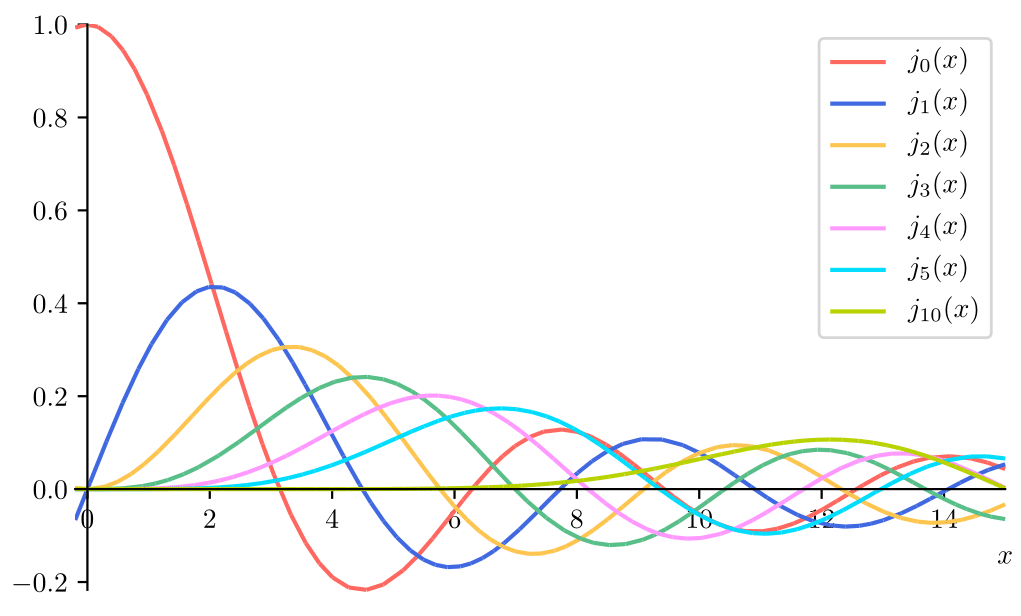
\includegraphics[width=75mm]{../fig/bessel/sph_j_n.png}
      \caption{球Bessel関数 $j_n(x)$}
    \end{figure}
 \end{minipage}

 \begin{minipage}{0.50\hsize}
    \begin{figure}[H]
      \centering
      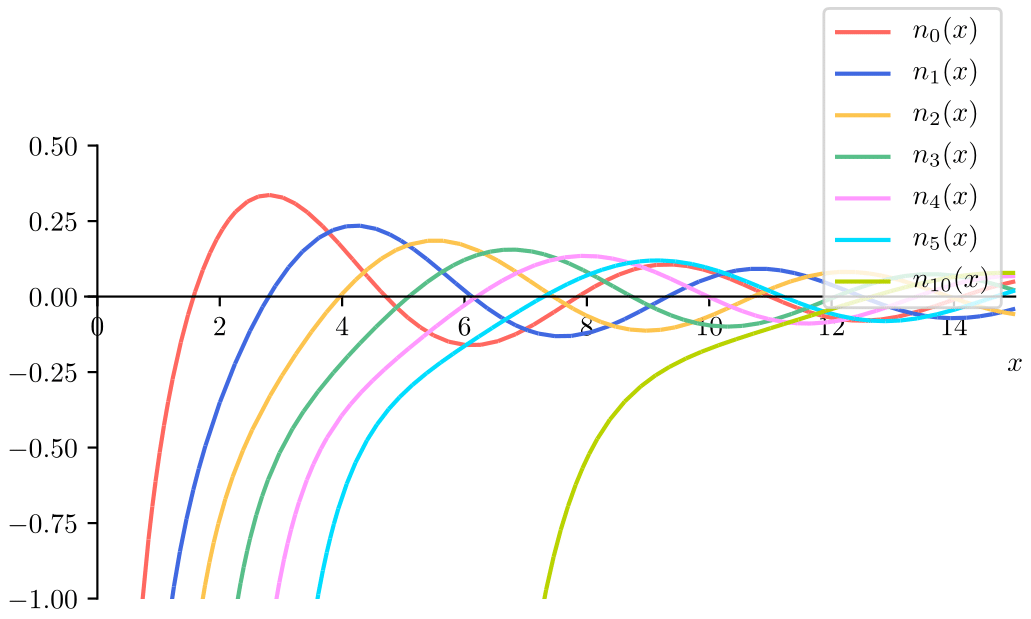
\includegraphics[width=75mm]{../fig/bessel/sph_n_n.png}
      \caption{球Neumann関数 $n_n(x)$}
    \end{figure}
 \end{minipage}
\end{tabular}
\end{figure}




\subsection*{証明}
以下の証明では任意の円柱関数$Z_\nu(x)$に対応する球Bessel関数を$z_n(x)$と書くことにする。

\paragraph{定義 $\Longrightarrow$ 一般項}
まず$j_n(x)$について、$J_\nu (x)$に関する一般項\eqref{eq:Jnu-ippan}を用いて
\begin{align*}
  j_n(x) &= \sqrt{\frac{\pi}{2x}} J_{n+\frac{1}{2}}(x)
	= \sqrt{\frac{\pi}{2x}} \sum_{i=0}^\infty \frac{(-1)^i}{i!\ \Gamma\(n +i+\frac{3}{2}\)} 
		\( \frac{x}{2} \)^{n+2i+\frac{1}{2}} \notag\\
	&= \frac{\sqrt{\pi}}{2} \sum_{i=0}^\infty \frac{(-1)^i}{i!\ \Gamma\(n +i+\frac{3}{2}\)} 
		\( \frac{x}{2} \)^{n+2i}
\end{align*}
ここでLegendreの倍数公式\eqref{eq:legendre-2z}
\footnote{\textbf{Legendreの倍数公式:}
\begin{equation}\label{eq:legendre-2z}
  \Gamma\( z+\frac{1}{2} \) = 2^{-2z+1} \sqrt{\pi} \ \frac{ \Gamma(2z)}{\Gamma(z)}
\end{equation}
}
を用いてガンマ関数の引数を整数にすると、
\begin{align*}
   j_n(x) 
	&=  \frac{\sqrt{\pi}}{2} \sum_{i=0}^\infty \frac{(-1)^i \ \Gamma(n+i+1)}
		{i! \cdot 2^{-2n-2i-1} \sqrt{\pi} \ \Gamma(2n+2i+2) } \( \frac{x}{2} \)^{n+2i} \notag\\
	&= 2^n x^n \sum_{i=0}^\infty \frac{(-1)^i (n+i)!}{i! \, (2n+2i+1)!} x^{2i}
\end{align*}

$n_n(x)$についても同様に$J_\nu (x)$に関する一般項\eqref{eq:Jnu-ippan}を用いて
\begin{align*}
  n_n(x) &= (-1)^{n+1} \sqrt{\frac{\pi}{2x}} J_{-n-\frac{1}{2}} (x)
	=  (-1)^{n+1} \sqrt{\frac{\pi}{2x}}  
		\sum_{i=0}^\infty \frac{(-1)^i}{i!\ \Gamma\(-n+i+\frac{1}{2}\)} \( \frac{x}{2} \)^{-n+2i-\frac{1}{2}}
	\notag\\
	&= (-1)^{n+1} \frac{\sqrt{\pi}}{x}
		\sum_{i=0}^\infty \frac{(-1)^i}{i!\ \Gamma\(-n+i+\frac{1}{2}\)} \( \frac{x}{2} \)^{-n+2i}
\end{align*}
Legendreの倍数公式\eqref{eq:legendre-2z}を用いてガンマ関数の引数を整数にすると、
\begin{align*}
  n_n(x) &= (-1)^{n+1} \frac{\sqrt{\pi}}{x}
		\sum_{i=0}^\infty \frac{(-1)^i \ \Gamma(-n+i)}{i!\cdot 2^{2n-2i+1} \sqrt{\pi} \ \Gamma(-2n+2i) } 
			\( \frac{x}{2} \)^{-n+2i} \notag\\
	&= \frac{(-1)^{n+1}}{2^{n+1} x^{n+1}}
		\sum_{i=0}^\infty \frac{(-1)^i \ \Gamma(-n+i+1)}
			{i!\ \Gamma(-2n+2i+1) } \cdot \frac{-2n+2i}{-n+i} \  x^{2i} \notag\\
	&= \frac{(-1)^{n+1}}{2^{n} \ x^{n+1}}
		\sum_{i=0}^\infty \frac{(-1)^i \ \Gamma(-n+i+1)}{i!\ \Gamma(-2n+2i+1) } x^{2i} \notag\\
\end{align*}
ここでガンマ関数を$\frac{(-n+i)!}{(-2n+2i)!}$のようにそのまま階乗に書き直すのは、
$i < n$の項において$\frac{\infty}{\infty}$の形が現れてしまい不適切である。
これを防ぐためには、$i\leq n \ (あるいは i < n)$の項に対して
次の公式を適用する
\footnote{
$\frac{\infty}{\infty}$が現れないようにするための手立てであるので、
$i \leq n$に対して適用しても$i < n$に対して適用しても式に意味を持たせることができる。
ここで二通りの書き方をあえて記述したのは、
次の「$x\sim 0$での振舞」を導く際には$i \leq n$に対して適用した\eqref{eq:nn-ippan}を、
「$x=0$の表式」を導くには$i < n$に対して適用した\eqref{eq:nn-ippan-2}を用いると分かりやすくなるからである。
\vspace{6pt}
 }
\footnote{
この証明にはガンマ関数の反射公式 $\Gamma(z) \Gamma(1-z) = \frac{\pi}{\sin\pi z}$を用いる。
いま階乗記号を$z! = \Gamma (z+1)$とガンマ関数の意味で用いることにすると、
この反射公式は$z!\ (-z)! = \frac{\pi z}{\sin \pi z}$と書き換えることができる。これより
\begin{equation*}
  \frac{(-n+i)!}{(-2n+2i)!}
	= \frac{(2n-2i)!}{(n-i)!} \cdot  \frac{\pi (n-i)}{\sin\pi (n-i)}  \cdot \frac{\sin \pi (2n-2i)}{\pi (2n-2i)}
	= \frac{(2n-2i)!}{(n-i)!} \cos \pi(n-i)
	= (-1)^{n-i} \frac{(2n-2i)!}{(n-i)!}
\end{equation*}
}
。
\begin{equation}
  \frac{(-n+i)!}{(-2n+2i)!}
	= (-1)^{n-i} \frac{(2n-2i)!}{(n-i)!}
\end{equation}
したがって、$n_n(x)$の一般項は次のように書ける:
\begin{align*}
  n_n(x) &= -\frac{1}{2^n x^{n+1}} \[ 
	\sum_{i=0}^{n} \frac{(2n-2i)!}{i! \, (n-i)!} x^{2i}
		+ (-1)^n \sum_{i=n+1}^\infty \frac{(-1)^i (-n+i)!}{i!\, (-2n+2i)!} x^{2i}
	 \] \notag\\
  &= -\frac{1}{2^n x^{n+1}} \[ 
	\sum_{i=0}^{n-1} \frac{(2n-2i)!}{i! \, (n-i)!} x^{2i}
		+ (-1)^n \sum_{i=n}^\infty \frac{(-1)^i (-n+i)!}{i!\, (-2n+2i)!} x^{2i} \]
\end{align*}\qed


\paragraph{一般項 $\Longrightarrow$ $x\sim 0$での振舞}
$x\sim 0$では一般項\eqref{eq:jn-ippan}, \eqref{eq:nn-ippan}において$i=0$の項が最も支配的になる。
まず$j_n(x)$について
\begin{equation*}
  j_n(x) \sim 2^n x^n \cdot \frac{n!}{(2n+1)!}
	= \frac{x^n}{(2n+1)!!} 
\end{equation*}
$n_n(x)$についても同様に
\begin{equation*}
  n_n(x) \sim - \frac{1}{2^n x^{n+1}} \cdot \frac{(2n)!}{n!} 
	= - \frac{(2n-1)!!}{x^{n+1}}
\end{equation*}\qed


\paragraph{一般項 $\Longrightarrow$ $n=0$の表式}
$j_n(x)$の一般項\eqref{eq:jn-ippan}で$n=0$とすると
\begin{equation*}
   j_0(x) = \sum_{i=0}^\infty \frac{(-1)^i}{(2i+1)!} x^{2i}
	= \frac{\sin x}{x}
\end{equation*}
同様に$n_n(x)$の一般項\eqref{eq:nn-ippan-2} で$n=0$とすると
\begin{equation*}
  n_0(x) = -\frac{1}{x} \sum_{i=0}^{\infty} \frac{(-1)^i}{(2i)!} x^{2i}
	= -\frac{\cos x}{x}
\end{equation*}
これらを用いると球Hankel関数についての式も直ちに得ることができ、
\begin{align*}
  h_0^{(1)}(x) &= j_0 (x) + i \, n_0(x) = \frac{\sin x}{x} - i \frac{\cos x}{x}
		= -\frac{i}{x} (\cos x + i\sin x) 
		= -i \frac{e^{ix}}{x} \notag\\
  h_0^{(2)} (x) &= j_0 (x) - i \, n_0(x)= \frac{\sin x}{x} + i \frac{\cos x}{x}
		= \frac{i}{x} (\cos x - i\sin x) 
		= i \frac{e^{-ix}}{x} 
\end{align*}
\qed

\paragraph{高階導関数表示}
$J_\nu(x)$についての高階導関数表示\eqref{eq:Jnu-kokai-1}において$\nu = \frac{1}{2}$とすると
\begin{equation*}
  x^{-n-\frac{1}{2}} J_{n+\frac{1}{2}} (x) = (-1)^n \( \frac{1}{x} \dx{} \)^n \[ x^{-\frac{1}{2}} J_\frac{1}{2}(x) \]
\end{equation*}
両辺を$\sqrt{\frac{\pi}{2}}x^n$倍すると
\begin{gather*}
  \sqrt{\frac{\pi}{2x}} J_{n+\frac{1}{2}} (x)
	= (-1)^n x^n \( \frac{1}{x} \dx{} \)^n \[ \sqrt{\frac{\pi}{2x}} J_\frac{1}{2} (x) \] \notag\\ \therefore
  j_n(x) = (-1)^n x^n \( \frac{1}{x} \dx{} \)^n j_0(x)
\end{gather*}
次に$J_\nu(x)$についての高階導関数表示\eqref{eq:Jnu-kokai-2}において$\nu = -\frac{1}{2}$とすると
\begin{equation*}
  x^{-n-\frac{1}{2}} J_{-n-\frac{1}{2}} (x) = \( \frac{1}{x} \dx{} \)^n \[ x^{-\frac{1}{2}} J_{-\frac{1}{2}}(x) \] 
\end{equation*}
両辺を$(-1)^{n+1} \sqrt{\frac{\pi}{2}} x^n$倍すると
\begin{gather*}
  (-1)^{n+1} \sqrt{\frac{\pi}{2x}} J_{-n-\frac{1}{2}} (x) 
	= (-1)^n x^n \( \frac{1}{x} \dx{} \)^n \[ - \sqrt{\frac{\pi}{2x}} J_{-\frac{1}{2}}(x) \]  \notag\\ \therefore
  n_n(x) =  (-1)^n x^n \( \frac{1}{x} \dx{} \)^n n_0(x)
\end{gather*}\qed

これらから球Hankel関数についての式も直ちに得ることができる。

\paragraph{漸化式}
円柱関数$Z_\nu(x)$についての漸化式\eqref{eq:Znu-req}において$\nu=n+\frac{1}{2}$とすると
\begin{equation*}
  \frac{2n+1}{x} Z_{n+\frac{1}{2}}(x) = Z_{n -\frac{1}{2}} (x) + Z_{n+\frac{1}{2}}(x)
\end{equation*}
よって両辺を$\sqrt{\frac{\pi}{2x}}$倍することで、定義より\eqref{eq:zn-req}が示される。\qed

\paragraph{微分漸化式}
球Bessel関数の定義を用いて$2\frac{d z_n(x)}{dx}$を展開すると、
\begin{align*}
  2\frac{d z_n(x)}{dx}
	&= 2 \dx{} \sqrt{\frac{\pi}{2x}} Z_{n+\frac{1}{2}} (x) \notag\\
	&= -\frac{1}{x} \sqrt{\frac{\pi}{2x}} Z_{n+\frac{1}{2}} (x)
		+ \sqrt{\frac{\pi}{2x}} \cdot 2 \frac{d Z_{n+\frac{1}{2}} (x)}{dx} \notag\\
	&= -\frac{1}{x} \sqrt{\frac{\pi}{2x}} Z_{n+\frac{1}{2}} (x)
		+ \sqrt{\frac{\pi}{2x}} \( Z_{n-\frac{1}{2}} (x) - Z_{n+\frac{3}{2}} (x) \) 
			\qquad (\eqref{eq:Znu-req-diff}を用いた)\notag\\
	&= -\frac{1}{x} z_n(x) + z_{n-1}(x) - z_{n+1} (x)
\end{align*}
移項して\eqref{eq:zn-req-diff}を得る。\qed

\paragraph{漸化式, 微分漸化式 $\Longrightarrow$ 昇降演算子}
下降演算子については$\frac{1}{2} \[ \eqref{eq:zn-req-diff} + \eqref{eq:zn-req} \]$を、
上昇演算子については$\frac{1}{2} \[ \eqref{eq:zn-req-diff} - \eqref{eq:zn-req} \]$を計算すると得られる。
\qed


\paragraph{昇降演算子 $\Longrightarrow$ 微分方程式}
下降演算子\eqref{eq:zn-kako}の両辺に$\( \dx{} - \frac{n-1}{x} \)$を左から作用させると左辺は
\begin{align*}
  &\hspace{-24pt}\( \dx{} - \frac{n-1}{x} \) \( \dx{} + \frac{n+1}{x} \) z_n(x) \notag\\
	&= \[ \dx{} \( \dx{} + \frac{n+1}{x} \) - \frac{n-1}{x} \( \dx{} + \frac{n+1}{x} \) \] z_n(x) \notag\\
	&= \[ \( \dx{2} - \frac{n+1}{x^2} + \frac{n+1}{x} \dx{} \)
		- \( \frac{n-1}{x} \dx{} + \frac{n^2-1}{x^2} \) \] z_n(x)  \notag\\
	&= \[ \dx{2} + \frac{2}{x}\dx{} - \frac{n(n+1)}{x^2} \] z_n(x) 
\end{align*}
一方右辺は$\( \dx{} - \frac{n-1}{x} \) z_{n-1}(x)$であるが、これは上昇演算子\eqref{eq:zn-josho}から
$-z_n(x)$に等しい。よって、
\begin{equation*}
  \[ \dx{2} + \frac{2}{x}\dx{} - \frac{n(n+1)}{x^2} \] z_n(x) = -z_n(x)  \qquad \therefore
  \frac{d^2 z_n(x)}{dx^2} + \frac{2}{x} \frac{d z_n(x)}{dx} 
	+ \[ 1- \frac{n(n+1)}{x^2} \] z_n(x) = 0
\end{equation*}
また、得られた微分方程式において$x\to kx$と置き換えると
\begin{equation*}
  \frac{d^2 z_n(kx)}{d(kx)^2} + \frac{2}{kx} \frac{d z_n(kx)}{d(kx)} 
	+ \[ 1- \frac{n(n+1)}{(kx)^2} \] z_n(kx) = 0
\end{equation*}
となり、
$\frac{d}{d(kx)} = \frac{1}{k} \dx{}$
に注意して整理すると\eqref{eq:zn-diff-eq2}が得られる。
さらに\eqref{eq:zn-diff-eq1}, \eqref{eq:zn-diff-eq2}はそれぞれ
\eqref{eq:zn-self-1}, \eqref{eq:zn-self-2}のようにも書ける。\qed


\paragraph{昇降演算子 $\Longrightarrow$ 微分・積分公式}
下降演算子\eqref{eq:zn-kako}の両辺に$x^{n+1}$をかけると

\begin{equation*}
  \[ x^{n+1} \dx{} + (n+1) x^{n} \] z_n(x) = x^{n+1} z_{n-1}(x) \qquad \therefore
	\dx{} [x^{n+1} J_z(x)] = x^{n+1} z_{n-1} (x)
\end{equation*}
これより積分公式は
\begin{equation*}
  \int x^{n+1} z_{n-1} (x) dx = x^{n+1} z_n(x) + C
\end{equation*}
同様に上昇演算子\eqref{eq:zn-josho}の両辺に$x^{-n}$をかけると
\begin{equation*}
  \( x^{-n} \dx{} - nx^{-n-1} \) z_n(x) = - x^{-n} z_{n+1}(x) \qquad \therefore
	\dx{} [x^{-n} z_n(x)] = -x^{-n} z_{n+1} (x) 
\end{equation*}
これより積分公式は
\begin{equation*}
  \qquad \int x^{-n} z_{n+1} (x) dx = - x^{-n} z_n(x) + C
\end{equation*}\qed

\subsection{球Bessel関数の直交性, Fourier-球Bessel展開}
Bessel関数の直交性\eqref{eq:Jnu-choko}において$\nu = l+\frac{1}{2}$を代入して整理することにより、
次の球Bessel関数の直交性を示すことができる
\footnote{
Bessel関数$J_{l+\frac{1}{2}} (x)$の正の零点
$\tilde{\alpha}_{l+\frac{1}{2}, 1}, \tilde{\alpha}_{l+\frac{1}{2}, 2}, \dots$が
球Bessel関数$j_l(x)$の正の零点$\alpha_{l1}, \alpha_{l2}, \dots $と一致することに注意して確認してみよ。
}
。

\begin{ibox}{球Bessel関数の直交性}
  球Bessel関数$j_l(x)$の正の零点を小さい順に
$\alpha_{l 1}, \alpha_{l 2}, \dots$とすると、次の直交性が成立する。
\begin{equation}\label{eq:jl-choko}
  \int_0^a x^2 \, j_l \(\frac{\alpha_{l m}}{a}x\) j_l \(\frac{\alpha_{l n}}{a}x \)dx
	= \frac{a^3}{2}\[ j_{l+1}(\alpha_{l n}) \]^2 \delta_{mn}
\end{equation}
\end{ibox}

さらに、球Bessel関数の直交性から、次のFourier-球Bessel展開も可能であることが分かる。
\begin{ibox}{Fourier-球Bessel展開}
  \noindent
  球Bessel関数$j_l(x) $の正の零点を小さい順に
  $\alpha_{l 1}, \alpha_{l 2}, \dots$とする。
  区間$[0, a]$で定義された関数$f(x)$がしかるべき条件を持つとき、
  関数$f(x)$は次のようにFourier-球Bessel展開できる。
  \begin{alignat}{2}
  &\textbf{展開式} && f(x) = \sum_{n=1}^\infty c_{l n} \, j_l \( \frac{\alpha_{l n}}{a} x \)  \\
  &\textbf{展開係数} &\quad & c_{l n} = \frac{2}{a^3 \[ j_{l+1} (\alpha_{l n}) \]^2} 
		\int_0^a x^2 f(x) j_l \( \frac{\alpha_{l n}}{a} x \) dx
\end{alignat}
\end{ibox}


\section{Bessel関数を使って解ける微分方程式}
物理系を記述する方程式としてBesselの微分方程式が現れた場合、
その基本解はいうまでもなくBessel関数になる。
しかしBesselの微分方程式と形が異なる方程式が現れたとき、
解法が確立されている形をしていたり、ほかのよく知られた特殊関数の微分方程式の形をしていたりしない限り、
その解がどうなるかは知る由もない。
ところがいくつかのケースにおいてはBessel関数に帰着できることが知られている。
次に示す処方箋は、この目安を与えるものである(問題[4-3])。

\begin{ibox}{Bessel関数を使って解ける微分方程式}
\noindent 微分方程式
\begin{equation}\label{eq:bessel-eq}
  y^{\prime\prime} + \( A_0 + \frac{A_1}{x} \) y^\prime 
		+ \( B_0 + \frac{B_1}{x} + \frac{B_2}{x^2} \) y = 0, \qquad A_0 A_1 = 2B_1
\end{equation}
の一般解は
\begin{equation}
  a = -\frac{A_0}{2}, \quad b = \frac{1-A_1}{2}, \quad 
	\nu = \sqrt{b^2-B_2}, \quad \gamma = \sqrt{B_0-a^2}
\end{equation}
を用いて次のようにBessel関数により表せる。
\begin{alignat}{2}
  & \nu \notin \mathbb{Z}のとき &\qquad &
  y = e^{ax} x^b \{ c_1 J_\nu (\gamma x) + c_2 J_{-\nu} (\gamma x) \} \\
  & 一般に &&
  y = e^{ax} x^b \{ c_1 J_\nu (\gamma x) + c_2 N_\nu (\gamma x) \}
\end{alignat}
ここで$\gamma$が純虚数であるときは$J_\nu (x), N_\nu (x)$の代わりに$I_\nu(x), K_\nu(x)$を用いる。
\end{ibox}

\begin{proof}
  Besselの微分方程式
  \begin{equation}\label{eq:Bess}
    \frac{d^2 Z_\nu (\gamma x)}{dx^2} + \frac{1}{x} \frac{d Z_\nu (\gamma x)}{dx}
	+ \( \gamma^2 - \frac{\nu^2}{x^2} \) Z_\nu (\gamma x) = 0
  \end{equation}
  に対して$Z_\nu (\gamma x) = e^{-ax} x^{-b} y$とおく。
  \begin{align*}
    &\frac{dZ_\nu (\gamma x)}{dx} = (-axy-by + xy^\prime) e^{-ax} x^{-b-1}\\
    &\frac{d^2 Z_\nu (\gamma x)}{dx^2} 
	= \[ a^2 x^2 y + b(b+1)y + x^2 y^{\prime\prime} + 2ab xy - 2bxy^\prime - 2ax^2y^\prime \]
		e^{-ax} x^{-b-2}
  \end{align*}
  であるので、\eqref{eq:Bess}にこれらを代入して整理すると
  \begin{equation*}
    y^{\prime\prime} + \( -2a + \frac{1-2b}{x} \) y^\prime
	+ \[ (a^2 + \gamma^2) + \frac{a(2b-1)}{x} + \frac{b^2- \nu^2}{x^2} \] y = 0
  \end{equation*}
  \eqref{eq:bessel-eq}と比較すると
  \begin{gather*}
    A_0 = -2a, \quad A_1 = 1-2b, \quad B_0 = a^2+\gamma^2, 
	\quad B_1 = a(2b-1), \quad B_2 = b^2-\nu^2 \notag\\\therefore
    a = -\frac{A_0}{2}, \quad b = \frac{1-A_1}{2}, \quad 
	\nu = \sqrt{b^2-B_2}, \quad \gamma = \sqrt{B_0-a^2}, \quad A_0A_1 = 2B_1
  \end{gather*}
  となる。
  また$\gamma$が虚数になるときは方程式\eqref{eq:Bess}が変形されたBesselの微分方程式と一致することから
  $J_\nu (x), N_\nu (x)$の代わりに$I_\nu(x), K_\nu(x)$を用いればよいことが分かる。
\end{proof}

\vspace{10pt}
\noindent \textbf{[例] 球Bessel微分方程式}

上記の処方箋を用いて球Bessel微分方程式
\begin{equation*}
  y^{\prime\prime} + \frac{2}{x} y^\prime 
	+ \[ k^2- \frac{n(n+1)}{x^2} \] y = 0
\end{equation*}
を解いてみよう。
\begin{equation*}
  A_0 = 0, \quad A_1 = 2, \quad B_0 = k^2, \quad B_1=0, \quad B_2=-n(n+1)
\end{equation*}
であるので$A_0 A_1 = 2B_1 = 0$を満たし、
\begin{equation*}
  a = -\frac{A_0}{2} = 0, \quad b = \frac{1-A_1}{2} = -\frac{1}{2}, \quad
	\nu = \sqrt{b^2-B_2} = n+\frac{1}{2} , \quad \gamma = \sqrt{B_0-a^2} = k
\end{equation*}
であるから、一般解は次のように書ける。
\begin{equation*}
  y = \frac{1}{\sqrt{x}} \left\{ C_1 J_{n+\frac{1}{2}} (kx) + C_2 N_{n+\frac{1}{2}} (kx) \right\}
\end{equation*}
ここで$C_1 = \sqrt{\frac{\pi}{2k}}c_1, \ C_2 = \sqrt{\frac{\pi}{2k}}c_2$とおきなおすと一般解は
\begin{equation*}
  y = c_1 j_n(kx) + c_2 n_n(kx)
\end{equation*}
となり、予想された球Bessel関数により記述できることが分かった。





\end{document}